% ============================================================
%  GamefyDB — PFE Report  |  Full Document
%  Compile with pdflatex (or XeLaTeX for UTF-8 support).
% ============================================================

\documentclass[12pt, a4paper]{report}

\usepackage[T1]{fontenc}
\usepackage[utf8]{inputenc}
\usepackage[english]{babel}
\usepackage{geometry}
\usepackage{graphicx}
\usepackage{hyperref}
\usepackage{booktabs}
\usepackage{array}
\usepackage{longtable}
\usepackage{enumitem}
\usepackage{titlesec}
\usepackage{fancyhdr}
\usepackage{xcolor}
\usepackage{listings}
\usepackage{caption}
\usepackage{subcaption}
\usepackage{float}
\usepackage{microtype}
\usepackage{amsmath}
\usepackage{tabularx}
\usepackage{multirow}
\usepackage{setspace}

\geometry{top=2.5cm, bottom=2.5cm, left=3cm, right=2.5cm}

\pagestyle{fancy}
\fancyhf{}
\fancyhead[L]{\small GamefyDB}
\fancyhead[R]{\small \leftmark}
\fancyfoot[C]{\thepage}
\renewcommand{\headrulewidth}{0.4pt}

\titleformat{\chapter}[display]
  {\normalfont\Large\bfseries\color{black}}
  {\chaptertitlename\ \thechapter}{10pt}{\Huge}
\titlespacing*{\chapter}{0pt}{-10pt}{20pt}

% ── Use-case description table style ─────────────────────────
\newcolumntype{L}{>{\raggedright\arraybackslash}p{3.5cm}}
\newcolumntype{R}{>{\raggedright\arraybackslash}p{10cm}}

\begin{document}

% ============================================================
%  TITLE PAGE
% ============================================================
\begin{titlepage}
\centering
\vspace*{1cm}

{\large Tunisian Republic}\\[0.3cm]
{\large Ministry of Higher Education and Scientific Research}\\[0.3cm]
{\large University of Monastir}\\[0.3cm]
{\large Higher Institute of Computer Science of Mahdia}\\[1.5cm]

% *TODO* insert your institution logo here
% \includegraphics[width=0.25\textwidth]{logo_isima.png}\\[1cm]

\vspace{1cm}
{\Large \textbf{Dissertation of Graduation}}\\[0.4cm]
{\normalsize Presented at the Higher Institute of Computer Science of Mahdia}\\[0.2cm]
{\normalsize Carried out at \textbf{Gamefy Academy, La Soukra, Tunis}}\\[0.8cm]

{\normalsize In view of obtaining the diploma of}\\[0.2cm]
{\large \textbf{Bachelor's Degree in Business Computing: Business Intelligence}}\\[1.2cm]

{\normalsize Prepared by:}\\[0.2cm]
{\Large \textbf{Sarra Mediouni}}\\[1.2cm]

{\LARGE \textbf{GamefyDB: Design and Development of an ETL Pipeline,}}\\[0.3cm]
{\LARGE \textbf{Data Warehouse, and Predictive Analytics System}}\\[0.3cm]
{\LARGE \textbf{for a Gaming Center}}\\[1.5cm]

% *TODO* insert defence date
{\normalsize Defended on \underline{\hspace{3cm}}}\\[1cm]

{\normalsize Before the jury composed of:}\\[0.5cm]
\begin{tabular}{ll}
  President:            & \textit{*TODO* jury president name and title} \\
  Reviewer:             & \textit{*TODO* reviewer name and title} \\
  Academic Supervisor:  & Mr.\ Sofien Boutaib \\
\end{tabular}\\[1cm]

{\normalsize Academic Year: 2025--2026}

\end{titlepage}

% ============================================================
%  DEDICATION
% ============================================================
\chapter*{Dedication}
\addcontentsline{toc}{chapter}{Dedication}
\thispagestyle{empty}

\vspace*{3cm}
\begin{center}
\itshape

% *TODO* write your personal dedication here. Below is a placeholder.

To my parents, for their unwavering support and patience throughout this journey.
To everyone who believed in this project before it was anything more than an idea.

\end{center}

\newpage

% ============================================================
%  ACKNOWLEDGEMENTS
% ============================================================
\chapter*{Acknowledgements}
\addcontentsline{toc}{chapter}{Acknowledgements}

I would first like to thank my academic supervisor, \textbf{Mr.\ Sofien Boutaib},
for his availability throughout the internship and for the time he put into
reviewing the written work. His feedback pushed me to be more precise in how I
justified technical decisions, particularly around the model selection and the
schema design choices.

I would also like to thank \textbf{Mr.\ Aymen Jadallah}, owner of Gamefy Academy,
for trusting me with access to the operational data and for taking the time to sit
through the sprint reviews. His comments were straightforward and grounded in how
the center actually runs, which was more useful than any requirements document would
have been. The Live Ops page in particular was redesigned almost entirely based on
his feedback after the first review session.

I am grateful to the jury members for taking the time to evaluate this work.

Finally, I thank my family for their support during what turned out to be a longer
and more complicated project than I had initially expected.

\newpage

% ============================================================
%  TABLE OF CONTENTS / FIGURES / TABLES
% ============================================================
\tableofcontents
\newpage
\listoffigures
\newpage
\listoftables
\newpage

% ============================================================
%  LIST OF ACRONYMS
% ============================================================
\chapter*{List of Acronyms}
\addcontentsline{toc}{chapter}{List of Acronyms}

\begin{tabular}{ll}
  \textbf{BI}    & Business Intelligence \\
  \textbf{ETL}   & Extract, Transform, Load \\
  \textbf{KPI}   & Key Performance Indicator \\
  \textbf{DW}    & Data Warehouse \\
  \textbf{DWH}   & Data Warehouse (alternative abbreviation) \\
  \textbf{EDW}   & Enterprise Data Warehouse \\
  \textbf{SQL}   & Structured Query Language \\
  \textbf{CSV}   & Comma-Separated Values \\
  \textbf{PK}    & Primary Key \\
  \textbf{FK}    & Foreign Key \\
  \textbf{DAX}   & Data Analysis Expressions \\
  \textbf{ML}    & Machine Learning \\
  \textbf{API}   & Application Programming Interface \\
  \textbf{UI}    & User Interface \\
  \textbf{PFE}   & Projet de Fin d'Études (Final Year Project) \\
  \textbf{PC}    & Personal Computer \\
  \textbf{PS5}   & PlayStation 5 \\
  \textbf{TND}   & Tunisian Dinar \\
  \textbf{UTF}   & Unicode Transformation Format \\
  \textbf{BOM}   & Byte Order Mark \\
  \textbf{NaN}   & Not a Number (missing value sentinel) \\
  \textbf{GIMSI} & Generalised Information Management System Integration \\
  \textbf{UML}   & Unified Modelling Language \\
  \textbf{VIP}   & Very Important Person \\
  \textbf{MoM}   & Month-over-Month \\
\end{tabular}

\newpage

% ============================================================
%  GENERAL INTRODUCTION
% ============================================================
\chapter*{General Introduction}
\addcontentsline{toc}{chapter}{General Introduction}

Gamefy Academy is a gaming center in La Soukra, Tunis, that has been running its
point-of-sale software since it opened. Every session, every transaction, every item
sold gets logged automatically. By the time I started my internship there, the owner
had months of Excel reports sitting on a local drive with no way to extract anything
useful from them. Decisions about staffing, stock ordering, and pricing were being
made without looking at any of that data --- not because the data was not there, but
because nothing had been built to process it. The goal of this project was to build
that system: an ETL pipeline to clean and structure the raw exports, a star-schema
data warehouse for Power~BI, interactive dashboards covering the key operational
KPIs, and a forecasting module to answer planning questions like how much stock to
order and which days need more staff.

The source data turned out to be far messier than it looked. Opening the Excel files
in a spreadsheet showed clean columns and readable numbers, but loading them
programmatically revealed encoding issues, non-standard number formats, and column
positions that shifted because of merged cells. Most of that was not visible from
the outside and none of it was documented. Dealing with it took up most of the
first two sprints.

The Scrum methodology was chosen to manage the project. In a data engineering
context where the shape of the problem reveals itself gradually as you inspect real
data, the ability to adapt between sprints matters more than having a rigid plan
from the beginning. Sprint~0 was used for planning. Four implementation sprints
followed, each adding a layer to the final system.

This report is structured around those sprints. Chapter~1 introduces the host
organisation, the existing system, and the proposed solution. Chapter~2 covers the
preparation work: requirements, backlog, architecture, and dimensional model.
Chapters~3 and~4 describe the ETL implementation, covering loading, cleaning, and schema
construction. Chapter~5 covers the Power~BI report. Chapter~6 covers the machine learning analytics module: forecasting, member
segmentation, and anomaly detection. A general conclusion summarises the outcomes
and suggests directions for future work.

\newpage

% ============================================================
%  CHAPTER 1
% ============================================================
\chapter{General Context of the Project}

\section{Introduction}

This first chapter sets up the rest of the report. It introduces the host gaming
centre, walks through the situation that motivated the work — what existed
before, what was missing, and what I proposed to build instead — and then
discusses how the project was managed and why I picked the methodology I did.

\section{Host Organisation Presentation}

\textbf{Gamefy Academy} is a gaming centre located in \textbf{La Soukra, Tunis}.
It opened in 2025 and targets a young clientele looking for a high-quality gaming
experience in a social setting. The centre offers PC gaming on high-end hardware,
two PlayStation~5 consoles, a private VIP gaming booth, and a small snack bar.
It positions itself in a market that has grown significantly in Tunisia over the
last few years, as competitive gaming and LAN events have become increasingly
popular.

% *TODO* insert Gamefy logo image if available
% \begin{figure}[H]
%   \centering
%   \includegraphics[width=0.3\textwidth]{images/gamefy_logo.png}
%   \caption{Gamefy Academy logo.}
% \end{figure}

\subsection{Organisational Structure}

Operations are run by a small team. Five cashier accounts handle all
customer-facing activity: \textit{taktek}, \textit{yassine}, \textit{youssef},
\textit{monta}, and \textit{guds}. A shared \textit{cashier} account is used during
shift hand-offs, and an \textit{admin} account is reserved for the owner. Each
cashier covers one or more terminals during a shift and is responsible for opening
sessions, ringing up snack purchases, and processing member top-ups.

Every customer-facing action is automatically logged by the centre's
point-of-sale software, which can export four Excel reports on demand: one for
cash transactions, one for gaming sessions, one for stock movements, and one for
the loyalty members.

\subsection{Services Provided}

The centre runs sixteen active terminals split across three categories:

\begin{itemize}
  \item \textbf{Standard PC workstations} (\textsc{GAMEFY01} to \textsc{GAMEFY10})
        — ten high-spec gaming computers. Sessions are billed by duration and
        marked as \textit{Standard}, \textit{Member}, \textit{Free},
        \textit{Time Limited}, or \textit{Administrator} depending on who is
        sitting at the terminal and why.

  \item \textbf{PlayStation~5 consoles} (\textsc{PS5\,(1)} and \textsc{PS5\,(2)})
        — two console stations managed the same way as the PCs.

  \item \textbf{VIP gaming booth} (\textsc{GAMEFY-VIP}) — a private room with a
        premium setup at a higher hourly rate, available by reservation.

  \item \textbf{Administrative workstations} (three \textsc{DESKTOP} machines) —
        used by staff for back-office work; they appear in the session data
        under the \textit{Administrator} type.
\end{itemize}

Alongside the gaming activity, the centre runs a snack bar stocked with drinks,
cookies, USB keys, and similar items. These sales are tracked through the stock
management system. A loyalty programme offers regular customers reduced rates and
keeps track of their cumulative spend and time.

\section{Project Presentation}

\subsection{General Context}

This project is the final-year work for the Bachelor's degree in Business
Computing with a Business Intelligence specialisation at the Higher Institute
of Computer Science of Mahdia (ISIMA), University of Monastir. The internship
ran over four months at Gamefy Academy, jointly supervised by an academic
supervisor from ISIMA and the centre's owner.

The project sits at the crossroads of data engineering and business analytics.
The starting point is four raw Excel files. The end goal is a repeatable system
that turns those files into clean data, into interactive dashboards, into
forward-looking forecasts, and finally into a conversational assistant the
owner can talk to in everyday language. None of that existed before the
internship started.

\subsection{Analysis of the Existing System}

When I arrived at Gamefy, the data workflow was simple: the point-of-sale
software exported four \texttt{.xls} files on demand and those files were saved
to a local folder. That was it. No pipeline processed them further. No dashboard
visualised them. If the owner wanted to know which cashier had had the best
month, which terminal was most popular, or whether revenue was trending up, the
only option was to open the right Excel file and build a pivot table by hand.

In practice that almost never happened. The friction of going from
``I have a question'' to ``I have an answer'' was high enough that analysis was
reserved for exceptional circumstances. The data accumulated but went unused.

\subsection{Criticism of the Current System}

Looking through the files in detail surfaced a second layer of problems beyond
the lack of tooling. The data-quality issues are invisible to someone reading
the spreadsheets in Excel, but they make automated processing much harder than
it should be. Table~\ref{tab:dq} summarises what I found.

\begin{table}[H]
  \centering
  \caption{Data-quality issues found in the source files.\label{tab:dq}}
  \begin{tabular}{p{3.5cm} p{9.5cm}}
    \toprule
    \textbf{Issue} & \textbf{Description} \\
    \midrule
    Page-break artefacts
      & The export software inserts a \textit{Page~X/Y} row, two blank rows, and
        a full header repetition roughly every 40 data rows. \\[4pt]
    Non-standard number format
      & TND amounts use a narrow no-break space (\texttt{\textbackslash u202f}
        / \texttt{\textbackslash xa0}) as the thousands separator and a comma
        as the decimal separator. Standard parsers reject both. \\[4pt]
    Merged-cell column shift
      & Merged cells in the Excel layout shift the column index where data
        actually lands relative to the visible header, so automatic header
        detection is unreliable. \\[4pt]
    Missing cashier names
      & Sub-total rows inserted between data rows carry a generic label in the
        cashier column instead of the actual account name. \\[4pt]
    Inconsistent totals
      & Some session and stock rows have recorded totals that do not match the
        sum of their component columns, pointing to data-entry or rounding
        errors in the source software. \\[4pt]
    Footer rows
      & The members file ends with a \textit{Report Result\,:} footer row that
        contains numeric totals in what looks like a data position. \\
    \bottomrule
  \end{tabular}
\end{table}

None of these issues were documented anywhere. Every one of them was discovered
by inspecting actual rows from the files and figuring out why the parser was
choking.

\subsection{Problem Statement}

Gamefy collects detailed operational data continuously, but derives almost no
value from it. The question this project addresses is therefore:
\textit{how can these raw, artefact-laden Excel exports be transformed reliably
and repeatably into a clean dataset that supports real decision-making, both
backward-looking and forward-looking?}

The word \textit{reliably} matters. A one-time manual clean is not a solution.
What the centre needs is a process that can be rerun every time the files
change, always producing correct output.

\subsection{Proposed Solution}

The solution I built is \textbf{GamefyDB}. It is a Python-based system that
covers four layers, all driven from a single command (\texttt{run.py}):

\begin{enumerate}
  \item \textbf{\texttt{gamefydb/pipeline.py}} handles the full ETL chain in one
        place: reading the four source files via \texttt{pandas}/\texttt{openpyxl},
        stripping every formatting artefact, correcting missing cashier names,
        converting every column to the right type, and finally building the
        six-table star schema (four dimensions and two facts). A single function,
        \texttt{run\_pipeline()}, runs the whole chain end-to-end.

  \item \textbf{\texttt{gamefydb/forecaster.py}} contains five independent
        forecasting functions plus an evaluation harness that compares
        \textbf{Prophet}, \textbf{SARIMA} (via \texttt{pmdarima.auto\_arima}),
        and \textbf{XGBoost} on an 80/20 chronological split. Two of those
        models also accept a \textbf{weather regressor} (daily max temperature
        and precipitation pulled from the Open-Meteo API and cached locally in
        \texttt{excel/weather\_tunis.parquet}).

  \item \textbf{\texttt{gamefydb/segmenter.py}} and
        \textbf{\texttt{gamefydb/anomaly\_detector.py}} produce the rest of the
        ML outputs: a K-Means segmentation of the member base into four
        behavioural profiles, a continuous loyalty score per member, and a
        day-of-week Z-score anomaly detector that flags revenue, session-volume,
        and member-activity outliers with a mild/severe severity label.

  \item \textbf{\texttt{app.py}} (Streamlit) is a conversational assistant that
        lets the owner ask questions in English, French, or Arabic, either by
        typing or by voice, and gets back a written answer plus a relevant
        chart. Four shortcut buttons (\textit{Full summary}, \textit{Give me
        advice}, \textit{Any anomalies?}, \textit{Forecast}) cover the most
        common queries in one click.
\end{enumerate}

The output of the ETL feeds into a Power~BI report (\texttt{gamefyyy.pbix})
with four dashboard pages — revenue overview, rankings, live ops, and shift
report — alongside the forecasting, segmentation, and anomaly CSVs. The
chatbot sits on top of the same data and uses the same forecasting/anomaly
functions internally.

Because the original source files only cover three months, I also built a
\textbf{synthetic data extension} (\texttt{gamefydb/data\_generator.py}) that
generates a longer history (\texttt{excel/extended\_*.xlsx}) by sampling from
the real daily-revenue pool and modulating it with Ramadan, Eid, monthly,
and weather-driven multipliers. Without this step the time-series models would
not have enough data to learn anything useful.

\section{Project Management Methodology}

Picking the right project management approach matters more than it looks. The
choice shapes how changes get handled, how progress is tracked, and how often
the stakeholder gets to see and react to what's been built. Below I look at
two methodologies commonly used in BI and software projects, then explain
which one I went with and why.

\subsection{The GIMSI Method}

GIMSI is a phased methodology designed specifically for decision-support and
Business Intelligence projects. It covers the full lifecycle, from the first
analysis of business needs all the way to operational deployment.

\subsubsection{GIMSI Objectives}

The method tries to:

\begin{itemize}[noitemsep]
  \item Organise the project work in a consistent, repeatable way.
  \item Keep the needs analysis, the design decisions, and the final deliverable
        aligned with each other.
  \item Tie the technical work back to the organisation's strategic goals.
  \item Capture the knowledge produced during the project so it can be reused
        later.
\end{itemize}

\subsubsection{Main Phases of GIMSI}

GIMSI splits the work into five sequential phases:

\begin{enumerate}[noitemsep]
  \item \textbf{Preliminary Study} — justify the project, analyse the context,
        identify the decision-making needs.
  \item \textbf{Opportunity Study} — assess feasibility and compare candidate
        solutions.
  \item \textbf{Detailed Study} — specify functional requirements and model the
        target system.
  \item \textbf{Implementation} — develop, integrate, and deploy.
  \item \textbf{Permanent Improvement} — refine the system based on operational
        feedback.
\end{enumerate}

\subsubsection{Advantages and Limits}

GIMSI's strength is that it combines top-down strategic framing with detailed
bottom-up technical work. Its phased structure reduces the risk of delivering
something that's technically correct but answers the wrong question. The
downside is that it does not handle moving targets well: it assumes that
business requirements are stable enough to specify upfront, which is rarely
the case in a data project where the source-data quality is unknown until
you open the files.

\subsection{Scrum Methodology}

Scrum is an agile framework built around short delivery cycles called sprints,
typically two to four weeks long. Each sprint ends with a working product
increment, a review with stakeholders, and a retrospective that feeds into
the next cycle.

\subsubsection{Key Principles}

Three roles define the team. The \textit{Product Owner} owns the backlog and
sets priorities based on business value. The \textit{Scrum Master} facilitates
the process and removes anything blocking the team. The \textit{Development
Team} is responsible for actually delivering each sprint's increment. The
ceremonies (Sprint Planning, Daily Scrum, Sprint Review, Sprint Retrospective)
create a rhythm that keeps everyone aligned and gives the stakeholder regular
visibility on progress without requiring a formal sign-off at every step.

\subsubsection{Advantages}

The biggest advantage of Scrum for a project like this one is the ability to
respond to change. When you discover during Sprint~1 that the source data has
half a dozen quality problems you did not know about before, Scrum lets you
fold those problems into the next sprint without derailing the plan.

\subsection{Adopted Methodology}

I went with \textbf{Scrum}. The deciding factor was uncertainty: when I started
the internship, I had no way of knowing what the data-quality issues were going
to be. Designing everything upfront would have meant making assumptions that
turned out to be wrong. Scrum let me inspect the real files in Sprint~1, fix
what I found, and only move on to the schema in Sprint~2 once the cleaning was
solid. Sprint~0 was used as a planning phase where no code was written. Five
implementation sprints followed.

\section{Conclusion}

Gamefy Academy had the data but not the infrastructure to use it. This chapter
identified the gap — messy files, no automation, no dashboard, no forecast,
no easy way for the owner to ask questions — and introduced the system built
to fill it. Chapter~2 covers the preparation work that was done before any
code was written.

% ============================================================
%  CHAPTER 2 — SPRINT 0: PREPARATION PHASE
% ============================================================
\chapter{Sprint 0: Preparation Phase}

\section{Introduction}

Sprint~0 is the planning sprint. Nothing ships at the end of it, but everything
that comes afterwards depends on getting it right. During this phase I
identified the actors, wrote down the requirements, set up the product
backlog, picked the technical architecture, and designed the dimensional
model. In practice the phase took longer than the two weeks originally
allocated, because understanding the source files well enough to write
reliable requirements meant looking at the real data in detail.

\section{Requirements Specification}

\subsection{Identification of System Actors}

GamefyDB interacts with three actors.

The \textbf{Gaming Centre Owner / Manager} is the main stakeholder. The owner
uses the Power~BI dashboards day-to-day, reads the forecasts and anomaly
alerts when planning ahead, and talks to the conversational assistant for
quick questions during a shift.

The \textbf{Data Analyst / BI Developer} is the role I played throughout the
internship. The analyst runs the pipeline, validates the output, maintains the
Power~BI report, and ships new ML or chatbot features as the requirements
evolve.

The \textbf{Cashier} is an indirect actor. Cashiers do not interact with
GamefyDB themselves, but their everyday activity generates the Excel exports
that the whole system depends on.

\subsection{Functional Requirements}

The functional requirements describe what the system must do. They were
derived from the problems in Chapter~1 and validated against the real source
files.

\begin{enumerate}
  \item Read the four source \texttt{.xls} files without triggering encoding
        errors.
  \item Strip every page-break artefact (repeated headers, \textit{Page X/Y}
        rows, blank rows) from each file before any processing.
  \item Parse TND amounts that use a narrow no-break space as the thousands
        separator and a comma as the decimal separator.
  \item Parse all datetime columns in \texttt{DD.MM.YYYY~HH:MM:SS} format
        into proper datetime objects.
  \item Convert duration strings in \texttt{Xh~Y~min} format into numeric
        minutes.
  \item Correct missing or invalid cashier names by propagating known cashier
        accounts through sub-total rows (\texttt{\_fill\_cashier}).
  \item Impute missing amounts and totals using the relationships between
        columns (e.g.\ \textit{total = quantity $\times$ unit~price}).
  \item Build four dimension tables with surrogate integer primary keys.
  \item Build two fact tables (\textit{fact\_transaction}, \textit{fact\_session})
        with foreign-key references resolved against the four dimensions.
  \item Export all six tables to \texttt{output/powerbi\_star/} as UTF-8-BOM
        encoded CSV files.
  \item Forecast revenue, member activity, peak hours/days, session volume,
        and stock replenishment using Prophet, SARIMA, and XGBoost on an
        80/20 chronological split, with the weather regressor available
        on Prophet and XGBoost.
  \item Segment the loyalty members into four behavioural profiles using
        K-Means clustering, and produce a continuous loyalty score per member.
  \item Flag days where revenue, session volume, or member activity was
        statistically unusual relative to the same day of the week, using a
        Z-score detector with a mild/severe severity label.
  \item Provide an interactive Power~BI report with at least four dashboard
        pages (revenue, rankings, live ops, shift report).
  \item Provide a Streamlit conversational assistant that supports English,
        French, and Arabic, accepts both text and voice input, and produces
        both a written answer and a relevant chart.
\end{enumerate}

\subsection{Non-Functional Requirements}

\begin{enumerate}
  \item \textbf{Correctness} — no artefact row, header row, or sub-total row may
        appear in any output table.
  \item \textbf{Reproducibility} — given the same four input files, the
        pipeline must always produce identical output.
  \item \textbf{Portability} — no hard-coded paths; the pipeline must run on
        any machine with the required Python packages, on both Windows and
        Linux.
  \item \textbf{Maintainability} — column index mappings are defined
        explicitly in each loader function so a format change in the source
        files can be corrected in one place.
  \item \textbf{Testability} — the parsing, cleaning, segmentation, anomaly,
        and weather modules are covered by an automated \texttt{pytest} suite.
\end{enumerate}

\subsection{Requirements Modelling}

Figure~\ref{fig:usecase} shows the global use case diagram for GamefyDB.

\begin{figure}[H]
  \centering
  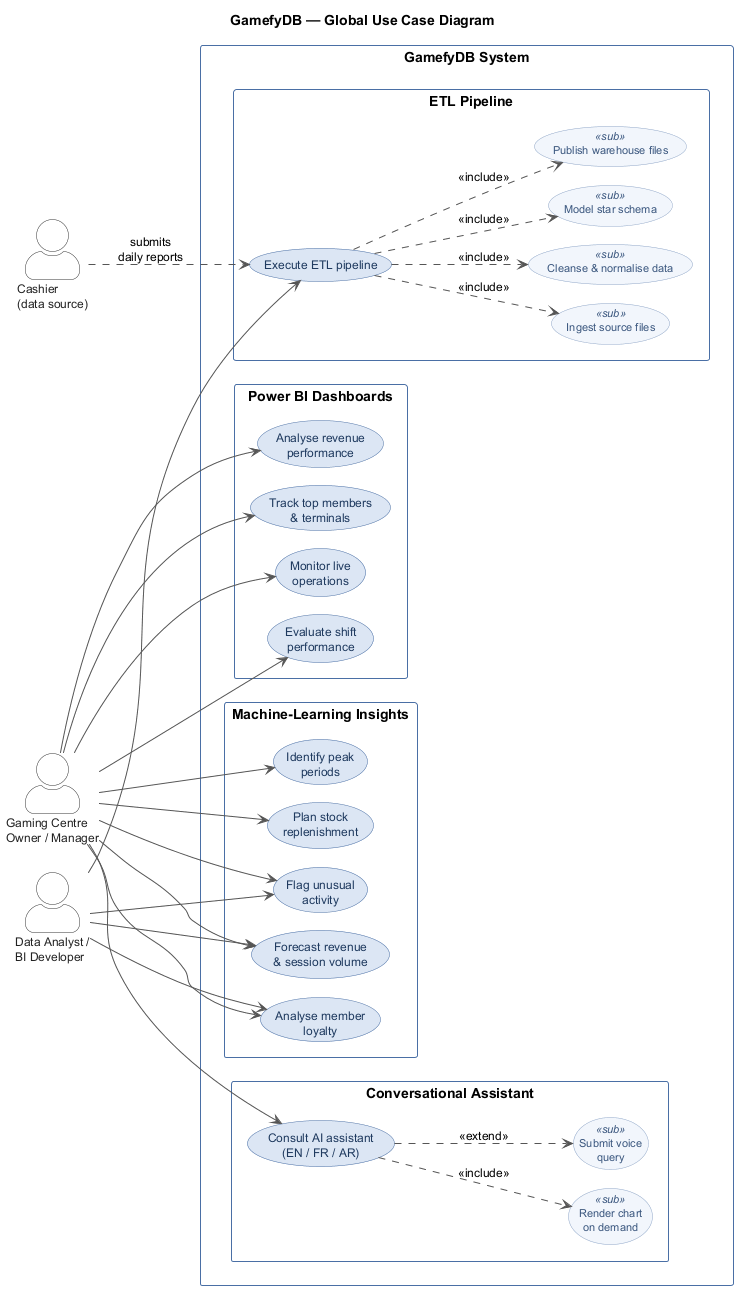
\includegraphics[width=0.95\textwidth]{images/use_cases.png}
  \caption{Global use case diagram for GamefyDB.}
  \label{fig:usecase}
\end{figure}

The three actors are stacked on the left of the system boundary; the
right-hand side groups the use cases into four packages that mirror the
project's four sprints: \textit{ETL Pipeline}, \textit{Power BI Dashboards},
\textit{Machine-Learning Insights}, and \textit{Conversational Assistant}.
The \textit{Cashier} is upstream of everything else: they generate the daily
exports that feed the pipeline, and only interact with the
\textit{Execute ETL pipeline} use case. The \textit{Analyst} triggers the
pipeline and drives the ML use cases (forecasts, segmentation, anomaly
detection). The \textit{Owner / Manager} is the broadest consumer: they
read every dashboard, every ML output, and query the conversational
assistant. Two composition patterns are visible on the right of the
diagram. \textit{Execute ETL pipeline} expands into its four sub-steps
(ingest, cleanse, transform, publish) via \texttt{<<include>>} arrows.
The conversational assistant always renders a chart on demand
(\texttt{<<include>>}) and optionally accepts a voice query
(\texttt{<<extend>>}).

\section{Project Management with Scrum}

\subsection{Identification of the Scrum Team}

\begin{itemize}
  \item \textbf{Product Owner}: \textbf{Mr.\ Aymen Jadallah}, owner of Gamefy
        Academy. He defined the business requirements, reviewed every sprint
        increment, and validated that the dashboards and the chatbot answered
        the kinds of questions he actually asks.

  \item \textbf{Scrum Master}: \textbf{Mr.\ Sofien Boutaib}, PhD in Computer
        Science from ISIMA and my academic supervisor. He made sure the Scrum
        ceremonies were respected and provided methodological and technical
        guidance throughout.

  \item \textbf{Development Team}: \textbf{Sarra Mediouni}, sole developer
        responsible for the pipeline, the ML modules, the Power~BI report,
        and the chatbot.
\end{itemize}

\subsection{Product Backlog}

The product backlog is the ordered list of every user story the project needs
to deliver. Sprint~4 (ML) and Sprint~5 (chatbot) were not in the original
backlog — they were added after Sprint~3 was validated, at the Product
Owner's request, once he could see what was possible on top of the cleaned
data.

\begin{longtable}{>{\bfseries}p{1.3cm} p{4.6cm} p{6.6cm} c}
  \caption{Product Backlog.\label{tab:backlog}} \\
  \toprule
  \textbf{ID} & \textbf{User Story} & \textbf{Tasks} & \textbf{Sprint} \\
  \midrule
  \endfirsthead
  \toprule
  \textbf{ID} & \textbf{User Story} & \textbf{Tasks} & \textbf{Sprint} \\
  \midrule
  \endhead
  \bottomrule
  \endfoot

  US-01 & As an analyst, I want to read all four source files without errors.
        & Implement one loader function per file in \texttt{pipeline.py};
          map column indices empirically.
        & 1 \\[3pt]
  US-02 & As an analyst, I want page-break artefacts removed automatically.
        & Implement \texttt{\_is\_header\_row()} and filter inside each loader.
        & 1 \\[3pt]
  US-03 & As an analyst, I want amounts, dates, and durations correctly typed.
        & Implement \texttt{\_parse\_amount()} and \texttt{\_parse\_duration()}.
        & 1 \\[3pt]
  US-04 & As an analyst, I want missing cashier names corrected.
        & Implement \texttt{\_fill\_cashier()} with forward/backward fill.
        & 1 \\[3pt]
  US-05 & As an analyst, I want four dimension tables with surrogate keys.
        & Build the dims inside \texttt{build\_star\_schema()}.
        & 2 \\[3pt]
  US-06 & As an analyst, I want two fact tables with FK references.
        & Build \textit{fact\_transaction} and \textit{fact\_session};
          resolve all FKs; use nullable \texttt{Int64} for optional refs.
        & 2 \\[3pt]
  US-07 & As an analyst, I want the schema exported as UTF-8-BOM CSV files.
        & Write the six tables to \texttt{output/powerbi\_star/} from
          \texttt{run.py}.
        & 2 \\[3pt]
  US-08 & As an owner, I want KPIs visualised in interactive dashboards.
        & Build \texttt{gamefyyy.pbix}: date dim, relationships, DAX measures,
          four dashboard pages.
        & 3 \\[3pt]
  US-09 & As an owner, I want a revenue forecast for the next 4 weeks and 3 months.
        & Implement \texttt{forecast\_revenue()} with Prophet.
        & 4 \\[3pt]
  US-10 & As an owner, I want to forecast member activity.
        & Implement \texttt{forecast\_members()} on weekly aggregates.
        & 4 \\[3pt]
  US-11 & As an owner, I want to see the busiest hours and days.
        & Implement \texttt{forecast\_peak\_hours()} returning two CSVs.
        & 4 \\[3pt]
  US-12 & As an owner, I want a forecast of total daily activity volume.
        & Implement \texttt{forecast\_session\_volume()} with Prophet.
        & 4 \\[3pt]
  US-13 & As an owner, I want a restocking recommendation per item.
        & Implement \texttt{forecast\_stock\_replenishment()}.
        & 4 \\[3pt]
  US-14 & As a data analyst, I want two more forecasting models for an
          objective comparison.
        & Implement SARIMA via \texttt{auto\_arima} and XGBoost with engineered
          features; evaluate Prophet vs SARIMA vs XGBoost on an 80/20
          chronological split (MAE, RMSE, wMAPE).
        & 4 \\[3pt]
  US-15 & As an owner, I want forecasts that take weather into account.
        & Add an Open-Meteo Tunis weather client (\texttt{weather.py});
          plug max-temperature + precipitation into Prophet and XGBoost as
          regressors.
        & 4 \\[3pt]
  US-16 & As an owner, I want to know which members are my most valuable.
        & Implement K-Means segmentation (k=4) in \texttt{segmenter.py};
          assign human-readable labels; export segments and per-member
          loyalty scores.
        & 4 \\[3pt]
  US-17 & As an owner, I want to be alerted on abnormally high or low days.
        & Implement day-of-week Z-score detection in
          \texttt{anomaly\_detector.py}; classify mild vs severe; export
          flagged dates to CSV.
        & 4 \\[3pt]
  US-18 & As an owner, I want to ask questions in plain language and get
          answers and charts back.
        & Build a Streamlit assistant (\texttt{app.py}); wire it to the
          star schema, the forecasts, the segments, and the anomalies.
        & 5 \\[3pt]
  US-19 & As an owner, I want to use the assistant in EN, FR, or AR.
        & Translate the UI strings and prompt the underlying agent in the
          selected language.
        & 5 \\[3pt]
  US-20 & As an owner, I want to talk to the assistant instead of typing.
        & Add a voice-input component to the Streamlit app
          (\texttt{chatbot/voice\_component.py}).
        & 5 \\[3pt]
  US-21 & As an owner, I want the assistant to draw a chart on demand.
        & Implement \texttt{chatbot/chart\_generator.py} so the agent can
          return a Plotly Express chart alongside a textual answer.
        & 5 \\
\end{longtable}

\subsection{Sprints Planning}

The project ran over five implementation sprints after Sprint~0:

\begin{itemize}
  \item \textbf{Sprint~1 — Data Loading and Cleaning}: the four loader
        functions, the artefact-filtering logic, the type-conversion helpers,
        and the cashier correction.
  \item \textbf{Sprint~2 — Star Schema and Export}: the dimensional model
        builder and the CSV export step, with referential-integrity checks
        across the six tables.
  \item \textbf{Sprint~3 — Power~BI Dashboards}: the full interactive report,
        the DAX measures, and KPI validation with the Product Owner.
  \item \textbf{Sprint~4 — Machine Learning and Analytics}: the five
        forecasting functions, the SARIMA / XGBoost comparison, the weather
        regressor, the K-Means segmentation, the loyalty score, and the
        Z-score anomaly detector.
  \item \textbf{Sprint~5 — Conversational Assistant}: the Streamlit chatbot
        with multilingual support (EN/FR/AR), voice input, and on-demand
        chart generation.
\end{itemize}

\subsection{Project Planning}

Table~\ref{tab:planning} shows the sprint schedule.

\begin{table}[H]
  \centering
  \caption{Sprint schedule.\label{tab:planning}}
  \begin{tabular}{lll}
    \toprule
    \textbf{Phase}  & \textbf{Start} & \textbf{End} \\
    \midrule
    Sprint 0 — Preparation                  & 02/02/2026 & 14/02/2026 \\
    Sprint 1 — Loading \& Cleaning          & 15/02/2026 & 02/03/2026 \\
    Sprint 2 — Star Schema \& Export        & 03/03/2026 & 12/03/2026 \\
    Sprint 3 — Power~BI Dashboards          & 13/03/2026 & 16/04/2026 \\
    Sprint 4 — ML and Analytics             & 17/04/2026 & 06/05/2026 \\
    Sprint 5 — Conversational Assistant     & 07/05/2026 & 17/05/2026 \\
    \bottomrule
  \end{tabular}
\end{table}

% *TODO* insert Gantt chart image here
% \begin{figure}[H]
%   \centering
%   
\includegraphics[width=\textwidth]{images/gantt.png}
%   \caption{Project Gantt chart.}
%   \label{fig:gantt}
% \end{figure}

\section{Technical Architecture}

Figure~\ref{fig:architecture} shows the overall architecture of the GamefyDB
solution.

\begin{figure}[H]
  \centering
  
\includegraphics[width=0.95\textwidth]{images/pipeline.png}
  \caption{Technical architecture of the GamefyDB solution.}
  \label{fig:architecture}
\end{figure}

The design is intentionally flat. The source layer is just the four Excel
files in \texttt{excel/} (plus a \texttt{weather\_tunis.parquet} cache and a
set of synthetic \texttt{extended\_*.xlsx} files used to give the time-series
models enough history). The processing layer is a handful of focused Python
modules — \texttt{pipeline.py} for the ETL, \texttt{forecaster.py} /
\texttt{segmenter.py} / \texttt{anomaly\_detector.py} for the ML layer,
\texttt{weather.py} for the regressor — all driven by \texttt{run.py}. The
output layer is two folders (\texttt{output/powerbi\_star/} for the star
schema and \texttt{output/forecasts/} for the ML outputs) that Power~BI and
the chatbot both read from directly.

Keeping the ETL in a single module rather than splitting it across four
ingest/clean/transform/export files was a deliberate choice. The cleaning
logic for each source file is tightly coupled to how that file is structured;
forcing it into a generic cleaner would have added abstraction without adding
clarity, and the column-index mappings are easier to maintain side by side
in one place.

\section{Overall Design of the Data Warehouse}

\subsection{Data Collection}

The source data is four \texttt{.xls} files exported by the centre's
point-of-sale software, covering activity from June~2025 through April~2026.
Table~\ref{tab:sourcefiles} summarises them.

\begin{table}[H]
  \centering
  \caption{Source files and their contents.\label{tab:sourcefiles}}
  \begin{tabular}{p{3.5cm} p{9cm}}
    \toprule
    \textbf{File} & \textbf{Contents} \\
    \midrule
    \texttt{14-06-2025 cash.xls}
      & One row per cash transaction. Columns include cashier, datetime,
        income/expense type, payment method, category, and TND amount. \\[4pt]
    \texttt{14-06-2025 session.xls}
      & One row per gaming session. Columns include cashier, terminal,
        session type, duration, and revenue broken down into usage, orders,
        USB data, and discount. \\[4pt]
    \texttt{14-06-2025 stock.xls}
      & One row per stock movement. Columns include cashier, datetime, item
        name, category, direction (in/out), quantity, unit price, and total. \\[4pt]
    \texttt{memeber DATA 01-09-2025.xls}
      & One row per loyalty member. Cumulative stats: total session duration,
        usage spend, order spend, USB spend, total spend. (The typo
        \textit{memeber} is in the real filename and is kept as-is.) \\
    \bottomrule
  \end{tabular}
\end{table}

\subsection{Key Performance Indicators (KPIs)}

The KPIs were defined during Sprint~0 in discussion with the Product Owner.
They fall into four groups for the descriptive side and one for the
forward-looking side. Table~\ref{tab:kpis} summarises them.

\begin{table}[H]
  \centering
  \caption{KPI groups and their measures.\label{tab:kpis}}
  \begin{tabular}{p{3cm} p{10cm}}
    \toprule
    \textbf{Group} & \textbf{KPIs} \\
    \midrule
    Revenue
      & Total income (TND), total expenses (TND), net income, revenue by
        payment method, revenue by cashier, revenue by transaction category,
        month-over-month revenue change, average transaction value. \\[4pt]
    Sessions
      & Total session count, average session duration (minutes), free-vs-paid
        split, total discount given, session revenue by terminal and by
        terminal type. \\[4pt]
    Stock
      & Total units sold per item, total snack-bar revenue, average unit
        price per item, current stock level. \\[4pt]
    Members
      & Active members, average spend per member, total session duration
        across all members, orders transferred, USB-data usage, loyalty score
        distribution. \\[4pt]
    Forward-looking
      & Revenue forecast (4~weeks / 3~months) with confidence interval,
        member-activity forecast, peak-hour and peak-day profile, per-item
        restocking recommendation, anomaly-flagged dates by series and
        severity. \\
    \bottomrule
  \end{tabular}
\end{table}

\subsection{Data Warehouse Design Approaches}

\subsubsection{Inmon Approach}

Bill Inmon's approach, often called \textit{top-down}, starts by designing a
single fully normalised enterprise data warehouse covering the whole
organisation, then derives subject-oriented data marts from it. Normalisation
keeps the redundancy low and gives a single source of truth, but it requires
the entire warehouse to be designed before any reports can be produced.

\subsubsection{Kimball Approach}

Ralph Kimball's approach, \textit{bottom-up}, models each business process as
an independent star schema and integrates them later through shared conformed
dimensions. It gets usable output into analysts' hands much faster, at the
cost of some potential redundancy between data marts.

\subsubsection{Adopted Approach}

I went with \textbf{Kimball}. With only four business domains, one physical
location, and a tight project timeline, designing a full normalised EDW
first would have taken the entire internship without producing any
dashboards. The bottom-up approach let me validate each output table against
the real data during Sprint~2 and adjust before moving on. The shared
\textit{dim\_cashier} and \textit{dim\_terminal} dimensions provide the
cross-domain integration that Kimball requires, without adding the complexity
of a fully normalised warehouse on top.

\section{Multidimensional Modelling}

\subsection{Conceptual Model Analysis}

Three dimensional schema patterns were evaluated:

\begin{itemize}
  \item \textbf{Star schema} — fact tables reference dimension tables directly,
        no further normalisation. Simple, fast, easy to understand. This is
        what Power~BI is optimised for.

  \item \textbf{Snowflake schema} — dimensions are further normalised into
        sub-dimensions. Saves some storage but adds joins at query time.
        Power~BI handles joins, but each extra one adds a little complexity
        to the model.

  \item \textbf{Galaxy (fact-constellation) schema} — multiple fact tables
        share conformed dimensions. This is essentially what GamefyDB needs,
        because both fact tables share the cashier, terminal, and member
        dimensions.
\end{itemize}

\subsection{Choice of Conceptual Model}

The model adopted is a \textbf{galaxy / fact-constellation schema}: two fact
tables (\textit{fact\_transaction} and \textit{fact\_session}) share three
conformed dimensions (\textit{dim\_cashier}, \textit{dim\_terminal},
\textit{dim\_member}), while \textit{dim\_item} is referenced from
\textit{fact\_transaction} only (for order-income rows). Stock movements and
per-member cumulative statistics were absorbed directly into the
\textit{dim\_item} and \textit{dim\_member} dimensions during the design
refinement of Sprint~2 — there is only one direction of stock movement
(out-of-stock sales) and the members file is cumulative rather than
event-based, so dedicated fact tables for them would have added complexity
without analytical value.

Figure~\ref{fig:starschema} shows the full conceptual model.

\begin{figure}[H]
  \centering
  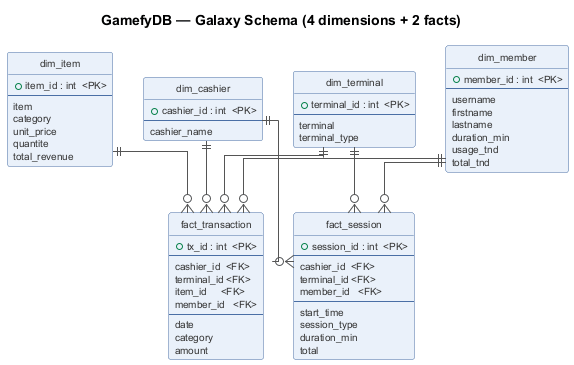
\includegraphics[width=\textwidth]{images/star_schema.png}
  \caption{Conceptual model of the GamefyDB data warehouse.}
  \label{fig:starschema}
\end{figure}

Table~\ref{tab:star_schema} lists the six output tables and their key columns.

\begin{table}[H]
  \centering
  \caption{Output tables of the GamefyDB star schema.\label{tab:star_schema}}
  \begin{tabular}{lll}
    \toprule
    \textbf{Type} & \textbf{Table} & \textbf{Key columns} \\
    \midrule
    Dimension & \texttt{dim\_cashier}  & cashier\_id (PK), cashier\_name \\
    Dimension & \texttt{dim\_terminal} & terminal\_id (PK), terminal, terminal\_type \\
    Dimension & \texttt{dim\_item}     & item\_id (PK), item, category, unit\_price, \\
              &                        & quantite, total\_revenue \\
    Dimension & \texttt{dim\_member}   & member\_id (PK), username, firstname, lastname, \\
              &                        & duration\_min, usage\_tnd, orders\_tnd, total\_tnd \\
    \midrule
    Fact & \texttt{fact\_transaction} & tx\_id (PK), cashier\_id (FK),
                                        terminal\_id (FK, nullable), \\
         &                            & item\_id (FK, nullable),
                                        member\_id (FK, nullable), \\
         &                            & date, category, amount \\
    Fact & \texttt{fact\_session}     & session\_id (PK), cashier\_id (FK),
                                        terminal\_id (FK), \\
         &                            & member\_id (FK, nullable),
                                        session\_type, duration\_min, \\
         &                            & order\_transfer, usage, discount, total \\
    \bottomrule
  \end{tabular}
\end{table}

\section{Work Environment}

\subsection{Hardware Environment}

\begin{itemize}[noitemsep]
  \item Machine: Lenovo laptop, model 83DV
  \item Processor: Intel Core i7-13650HX (13th gen), 14 cores / 20 threads
  \item RAM: 32~GB
  \item Storage: 500~GB MSI M450 SSD + 512~GB Micron NVMe SSD
  \item GPU: NVIDIA GeForce RTX 4050 Laptop
  \item Operating system: Windows~11 Pro
\end{itemize}

\subsection{Software Environment}

\begin{itemize}
  \item \textbf{Python 3.x} — main implementation language for the pipeline,
        the ML modules, the chatbot, and the helper scripts.
  \item \textbf{pandas} and \textbf{NumPy} — used throughout for reading the
        source files, all DataFrame operations, vectorised nearest-neighbour
        FK matching, and CSV/Excel output.
  \item \textbf{openpyxl} — reads and writes the \texttt{.xlsx} extended files
        produced by the synthetic data generator.
  \item \textbf{Prophet} (Meta) — additive time-series model used to forecast
        revenue, member activity, and session volume, with the Open-Meteo
        weather regressor.
  \item \textbf{pmdarima} — wraps an \texttt{auto\_arima} SARIMA fitting
        routine used as the comparison baseline for Prophet.
  \item \textbf{XGBoost} — gradient-boosting model used as a third
        comparison algorithm, with engineered lag and weather features.
  \item \textbf{statsmodels} — provides the Augmented Dickey-Fuller test
        used for the stationarity study in Sprint~4.
  \item \textbf{scikit-learn} — provides K-Means and the preprocessing
        utilities used by the member segmentation.
  \item \textbf{matplotlib} — generates all the accuracy, segmentation,
        peak-hour, and anomaly-timeline figures shipped with the report.
  \item \textbf{requests} — calls the Open-Meteo API for daily Tunis weather
        and caches the result in a parquet file.
  \item \textbf{Streamlit} — runs the conversational assistant
        (\texttt{app.py}), including the multilingual UI and the voice-input
        component.
  \item \textbf{Power~BI Desktop} — loads the star schema and the analytics
        CSVs, defines the relationships, writes the DAX measures, and assembles
        the four-page interactive report (\texttt{gamefyyy.pbix}).
  \item \textbf{pytest} — automated testing for the parsing, cleaning,
        segmentation, anomaly, and weather modules.
  \item \textbf{VS~Code} — code editor with the Python and PlantUML extensions.
  \item \textbf{PlantUML} — diagramming tool used to generate the use-case,
        pipeline-architecture, and star-schema diagrams from
        \texttt{.puml} sources.
  \item \textbf{Git / GitHub} — version control and remote repository hosting
        for all code and documentation.
  \item \textbf{Overleaf} — online \LaTeX{} editor used to write and compile
        this report.
\end{itemize}

\section{Conclusion}

By the end of Sprint~0, the scope was defined, the backlog was in place,
and the architectural decisions had been made. The choice of Kimball over
Inmon, galaxy schema over snowflake, and one unified pipeline module over
separate stage files all came from the same place: the project is small,
the data quality is uncertain, the timeline is short, and adding abstraction
upfront would have slowed everything down without paying for itself.
Chapter~3 covers the first implementation sprint, where the loading and
cleaning work actually started.

% ============================================================
% ============================================================
%  CHAPTER 3
% ============================================================
\chapter{Sprint 1: Data Loading and Cleaning}

\section{Introduction}

This sprint covers the loading and cleaning of the four source files. The scope
includes removing formatting artefacts, parsing columns into the correct types,
imputing missing values, and correcting cashier names. It corresponds to user
stories US-01 through US-04.

This sprint took longer than expected. The source files turned out to have more
problems than were visible from a first inspection, and several issues were only
discovered after earlier fixes revealed new ones underneath. That discovery process
is part of what made Scrum the right methodology: each sprint ended with a validated
result, which meant the next sprint started from a solid base.

All code for this sprint lives in \texttt{gamefydb/pipeline.py}.

\section{Sprint 1 Backlog}

\begin{longtable}{>{\bfseries}p{1.3cm} p{4.2cm} p{7cm}}
  \caption{Sprint 1 Backlog.\label{tab:sprint1_backlog}} \\
  \toprule
  \textbf{ID} & \textbf{User Story} & \textbf{Tasks} \\
  \midrule
  \endfirsthead
  \toprule
  \textbf{ID} & \textbf{User Story} & \textbf{Tasks} \\
  \midrule
  \endhead
  \bottomrule
  \endfoot

  US-01 & Read all four source files without errors.
        & Implement \texttt{load\_and\_clean\_cash()},
          \texttt{load\_and\_clean\_sessions()},
          \texttt{load\_and\_clean\_stock()}, and
          \texttt{load\_and\_clean\_members()}.\\[4pt]
  US-02 & Remove all page-break artefacts automatically.
        & Implement and apply \texttt{\_is\_header\_row()} in every loader. \\[4pt]
  US-03 & Parse amounts, dates, and durations correctly.
        & Implement \texttt{\_parse\_amount()} and \texttt{\_parse\_duration()}. \\[4pt]
  US-04 & Correct missing cashier names.
        & Implement \texttt{\_fill\_cashier()} with forward/backward fill. \\
\end{longtable}

\section{Use Case Analysis}

Table~\ref{tab:uc_clean} gives the text description of the main use case for this
sprint.

\begin{table}[H]
\centering
\caption{Text description of use case ``Load and Clean Source Files''.\label{tab:uc_clean}}
\begin{tabular}{L R}
  \toprule
  \textbf{Field} & \textbf{Description} \\
  \midrule
  Use Case Name  & Load and Clean Source Files \\
  Actor          & Data Analyst \\
  Preconditions  & All four \texttt{.xls} files are present in the \texttt{excel/}
                   directory. \\
  Main Flow      & 1. \texttt{run\_pipeline()} is called with the input directory. \newline
                   2. Each of the four loader functions is called in sequence. \newline
                   3. Each loader reads its file with \texttt{pandas.read\_excel}. \newline
                   4. Artefact rows are removed using \texttt{\_is\_header\_row()}. \newline
                   5. Columns are selected by index and renamed. \newline
                   6. Types are converted: amounts, datetimes, durations. \newline
                   7. Missing values are imputed where rules apply. \newline
                   8. Cashier names are corrected with \texttt{\_fill\_cashier()}. \newline
                   9. The cleaned DataFrame is returned. \\
  Alternative Flow & If a value cannot be parsed (e.g.\ a malformed amount), it is
                   set to NaN and either imputed from related columns or filled
                   with the category median. \\
  Postconditions & Four clean, fully typed DataFrames with no artefact rows,
                   no missing mandatory values, and correct cashier names on all
                   rows. \\
  \bottomrule
\end{tabular}
\end{table}

% *TODO* insert sequence diagram for the loading process
% \begin{figure}[H]
%   \centering
%   \includegraphics[width=\textwidth]{seq_loading.png}
%   \caption{Sequence diagram for the loading and cleaning process.}
%   \label{fig:seq_loading}
% \end{figure}

\section{Reading the Source Files}

\subsection{Why Column Indices Are Hardcoded}

All four files are read with \texttt{pandas.read\_excel(path, header=None)}, loading
the entire sheet as a raw DataFrame with numeric column indices. Automatic header
detection cannot be used here because Excel's merged cells shift where the data
lands relative to the visible headers.

For example, in the cash file the header for the transaction category column appears
at one index, but the actual category values for data rows are at a different one.
The only way to know the correct position is to inspect real data rows. I did this
for all four files and recorded the correct positions in a \texttt{COLS} dictionary
at the top of each loader function.

This is the most brittle part of the pipeline. If the point-of-sale software ever
changes its export format, these indices will need to be re-verified. That is
documented in the code.

\subsection{Removing Artefact Rows}

The export software inserts a page-break sequence every 40 rows or so. The sequence
is: a \textit{Page~X/Y} label, two blank rows, then a complete repetition of all
column headers. The \texttt{\_is\_header\_row()} function catches them by checking
three conditions: the value is empty, the value equals the literal string
``Cashier'' (the first column header in all files), or the value matches the
date-like pattern that appears in page-marker rows. Any row that triggers this on
its key column is dropped before any other processing.

\section{Parsing Helpers}

\subsection{Monetary Amounts}

The TND amount format is the most unusual issue in the files. A value like
\texttt{1 745,44 TND} looks normal in Excel, but the space between 1 and 745 is a
narrow no-break space (Unicode \texttt{U+202F}), not a regular space. Python's
standard \texttt{float()} function rejects it.

The \texttt{\_parse\_amount()} function handles this by stripping all whitespace
variants, removing the TND suffix, converting the comma decimal separator to a period,
and then converting to float. If the result still cannot be converted, \texttt{NaN}
is returned and handled downstream.

\subsection{Session Durations}

Durations are stored as human-readable strings: \texttt{1h 29 min}, \texttt{30 min},
or occasionally just a number. The \texttt{\_parse\_duration()} function splits on
the \texttt{h} separator if present, converts hours to minutes, adds the remainder,
and returns a float representing total minutes. The result is used in Power~BI
for average session duration calculations.

\section{Per-File Cleaning}

Table~\ref{tab:file_issues} summarises what was found in each file and how it was
handled.

\begin{table}[H]
  \centering
  \caption{Per-file cleaning summary.\label{tab:file_issues}}
  \begin{tabular}{p{2.5cm} p{4cm} p{6cm}}
    \toprule
    \textbf{File} & \textbf{Issues found} & \textbf{Solution} \\
    \midrule
    Cash
      & Missing income/expense type; missing amounts; missing dates;
        missing payment method.
      & Type imputed from category map; amounts filled with category
        median; dates forward-filled; payment defaulted to Cash. \\[4pt]
    Sessions
      & Sub-total rows for terminal types and summary rows for amounts;
        recorded totals not matching sum of components.
      & Noise labels filtered explicitly; total recomputed from
        usage + orders + USB $-$ discount where discrepancy exceeds 0.01 TND. \\[4pt]
    Stock
      & Occasional missing quantity, unit price, or total (one of three
        values sometimes absent); recorded totals inconsistent.
      & Mutual imputation from the two present values; total recomputed
        from quantity $\times$ unit price. \\[4pt]
    Members
      & Footer row \textit{Report Result\,:} with numeric totals in data
        position; missing first names; inconsistent total column.
      & Member ID coerced to numeric; the footer fails and is dropped; first
        name filled from username; total recomputed. \\
    \bottomrule
  \end{tabular}
\end{table}

\subsection{Cash Transactions}

After artefact removal, the cash loader applies four corrections in sequence. First,
rows missing the income/expense flag have it inferred from the category column using
a lookup dictionary, for example \textit{Computer Incomes} maps to \textit{Income}
and \textit{Discounts} maps to \textit{Expense}. Second, rows with a missing amount
are filled using the median amount for their category, so they are not simply dropped
and excluded from aggregations. Third, rows with a missing date are forward-filled,
since consecutive rows from the same session always share a timestamp. Fourth, null
payment values are set to \textit{Cash}, the default payment method at the center.

\subsection{Gaming Sessions}

The sessions file has more noise than the others. In addition to the standard
page-break artefacts, it contains sub-total rows (one per terminal type, one per
summary metric) that carry labels like \textit{Computer}, \textit{Total},
\textit{Orders Amount}, and so on. A set of known noise labels is defined in the
code. Any row whose cashier, terminal, or session-type field matches a label in that
set is dropped.

After filtering, each terminal gets a type assigned based on its name: anything
containing \texttt{PS5} is a PlayStation station, anything containing \texttt{VIP}
is a VIP PC, and everything else is a Standard PC. The session total is then
validated against the sum of its components. If the discrepancy exceeds 0.01 TND
(which happens on a small number of rows, likely due to rounding differences in the
source software), the recorded total is replaced with the computed one.

\subsection{Stock Movements}

The stock file is relatively well-structured. After artefact removal and type
parsing, a mutual-imputation step handles rows where one of the three financial
columns is missing: quantity, unit price, or total. If any two of the three are
present, the third is computed from them. Then the total is validated against
quantity times unit price, the same way as in the sessions file.

\subsection{Member Statistics}

The members file has two issues beyond the standard ones. The footer row at the end
of the file is the most subtle: it looks like a data row because it has a numeric
value in the member ID column position. The fix is simple but non-obvious: coercing
the member ID to a proper integer and dropping any row where this fails removes it
cleanly. The second issue is missing first names: where the first name field is
empty or contains \textit{nan}, it is replaced with the member's username, which is
always present.

\section{Fixing Cashier Names}

The cashier naming problem deserves a separate section because it affects all three
transactional files and the fix is not completely obvious.

The point-of-sale software inserts sub-total rows periodically (one row per shift,
per terminal type, or per summary category) and these rows carry a generic label
in the cashier column. The labels vary: sometimes it is the terminal type name,
sometimes it is a session category, sometimes it is a reporting label. The only
consistent property is that none of them match the five real cashier account names:
\textit{guds}, \textit{monta}, \textit{taktek}, \textit{yassine}, \textit{youssef}.

The \texttt{\_fill\_cashier()} function uses this. It sets any value in the cashier
column that is not in the known-cashiers list to \texttt{NaN}, then applies a forward
fill followed by a backward fill. The forward fill propagates the most recent real
cashier name to all subsequent sub-total rows. The backward fill handles any leading
sub-total rows that appear before the first real cashier entry.

\section{Sprint 1 Review}

\subsection{Deliverables}

The sprint produced four working loader functions in \texttt{gamefydb/pipeline.py}
and a \texttt{pytest} test suite covering the two parsing helpers and the cashier
fill logic with edge cases.

\subsection{Validation}

Each loader was run against the real source files. The validation checks were:

\begin{itemize}[noitemsep]
  \item Row counts after artefact removal matched the expected data rows.
  \item No \texttt{NaN} values remained in any mandatory column.
  \item \texttt{dtypes} confirmed correct types across all columns.
  \item Session totals matched recomputed values within 0.01 TND.
  \item Stock totals matched quantity times unit price within 0.01 TND.
  \item All cashier values in every file were from the known-cashiers list.
\end{itemize}

\section{Conclusion}

Sprint~1 handled the messiest, least visible part of the project. The cleaning
work is not glamorous, but everything that comes after depends on it being correct.
A single row with a wrong type or a stray sub-total can propagate errors through
the entire schema. Chapter~4 covers how the clean DataFrames are assembled into
the star schema.

% ============================================================
%  CHAPTER 4
% ============================================================
\chapter{Sprint 2: Star Schema and Data Export}

\section{Introduction}

Sprint~2 takes the four clean DataFrames from Sprint~1 and turns them into the six
output tables that make up the GamefyDB star schema. It also handles writing those
tables to disk in a format Power~BI can read. The sprint covers user stories US-05
through US-07, and by the end of it the full pipeline is working end to end.

\section{Sprint 2 Backlog}

\begin{longtable}{>{\bfseries}p{1.3cm} p{4.2cm} p{7cm}}
  \caption{Sprint 2 Backlog.\label{tab:sprint2_backlog}} \\
  \toprule
  \textbf{ID} & \textbf{User Story} & \textbf{Tasks} \\
  \midrule
  \endfirsthead
  \toprule
  \textbf{ID} & \textbf{User Story} & \textbf{Tasks} \\
  \midrule
  \endhead
  \bottomrule
  \endfoot

  US-05 & Build four dimension tables with surrogate keys.
        & Build \textit{dim\_cashier}, \textit{dim\_terminal}, \textit{dim\_item},
          and \textit{dim\_member} inside \texttt{build\_star\_schema()}. \\[4pt]
  US-06 & Build two fact tables with FK references.
        & Build \textit{fact\_transaction} and \textit{fact\_session}; resolve
          all FK references; nullable Int64 for optional refs. \\[4pt]
  US-07 & Export the schema as CSV files for Power~BI.
        & Write all six tables to \texttt{output/powerbi\_star/} with UTF-8-BOM. \\
\end{longtable}

\section{Use Case Analysis}

\begin{table}[H]
\centering
\caption{Text description of use case ``Build Star Schema''.\label{tab:uc_schema}}
\begin{tabular}{L R}
  \toprule
  \textbf{Field} & \textbf{Description} \\
  \midrule
  Use Case Name  & Build Star Schema \\
  Actor          & Data Analyst (via \texttt{run.py}) \\
  Preconditions  & The four loader functions have been called and returned clean
                   DataFrames with no artefact rows and correct types. \\
  Main Flow      & 1. All distinct cashier names are collected from the three
                      transactional files and sorted. \newline
                   2. \textit{dim\_cashier} is built with sequential surrogate keys. \newline
                   3. \textit{dim\_terminal} is built from unique (name, type) pairs
                      in the sessions data. \newline
                   4. Stock data is aggregated per item to build \textit{dim\_item}. \newline
                   5. The cleaned members DataFrame becomes \textit{dim\_member}. \newline
                   6. \textit{fact\_transaction} is built from the cash data with
                      FK references resolved. \newline
                   7. \textit{fact\_session} is built from the sessions data. \newline
                   8. All six tables are returned as a dictionary. \\
  Alternative Flow & If a cashier name in a fact table has no match in the dimension,
                   the FK is set to NaN rather than raising an error. \\
  Postconditions & Six correctly keyed tables with no orphaned foreign keys. \\
  \bottomrule
\end{tabular}
\end{table}

% *TODO* insert sequence diagram for schema building
% \begin{figure}[H]
%   \centering
%   \includegraphics[width=\textwidth]{seq_schema.png}
%   \caption{Sequence diagram for the star schema construction.}
%   \label{fig:seq_schema}
% \end{figure}

\section{A Design Change}

The Sprint~0 backlog described eight output tables. During Sprint~2 I revisited this
after looking more carefully at what the stock and members data actually contained.

The stock file only records outgoing sales. There are no incoming stock entries in
the entire dataset. A fact table with a single movement direction adds no analytical
value beyond what an aggregated dimension can provide. So the stock data was absorbed
into \textit{dim\_item}: total quantity sold and total revenue per item are stored
as item attributes, alongside the median unit price and category.

The members file already contains one summary row per member, with cumulative totals
rather than individual events. That is not a fact table, it is a dimension. Treating
it as a fact table would mean every report involving members requires an additional
aggregation that the data does not actually need.

The result is six tables instead of eight. All the planned KPIs are still computable;
the model is just simpler.

\section{Building the Dimension Tables}

\subsection{dim\_cashier}

All distinct cashier names are collected from the cash, sessions, and stock
DataFrames, sorted alphabetically, and assigned sequential surrogate keys starting
at~1. The resulting dimension has five rows, one per cashier account.

\subsection{dim\_terminal}

The terminal dimension is built from the sessions file only, since it is the only
source that records terminal names consistently and completely. Each unique
combination of terminal name and terminal type produces one row. There are 16
terminals in total, split as shown in Table~\ref{tab:terminals}.

\begin{table}[H]
  \centering
  \caption{Terminal type breakdown.\label{tab:terminals}}
  \begin{tabular}{lr}
    \toprule
    \textbf{Terminal type} & \textbf{Count} \\
    \midrule
    Standard PC & 10 \\
    PlayStation & 2 \\
    VIP PC      & 1 \\
    Administrative (DESKTOP) & 3 \\
    \bottomrule
  \end{tabular}
\end{table}

\subsection{dim\_item}

The stock DataFrame is grouped by item name. For each item, the dimension stores
the first observed category, the median unit price across all transactions, the total
quantity sold, and the total revenue. Median is used rather than mean for the unit
price so that occasional data-entry errors do not distort the reference price.
Seventeen distinct items appear in the data.

\subsection{dim\_member}

The cleaned members DataFrame is used directly as the member dimension. It has 66
rows, one per loyalty member, with name fields, cumulative session duration in
minutes, and spending broken down by usage, orders, USB data, and total.

\section{Building the Fact Tables}

\subsection{fact\_transaction}

Each row in this table is one cash register event. The foreign key resolution is
selective: not every transaction references every dimension. Table~\ref{tab:fk_rules}
shows the rules.

\begin{table}[H]
  \centering
  \caption{Foreign key assignment rules for \textit{fact\_transaction}.\label{tab:fk_rules}}
  \begin{tabular}{p{3cm} p{9.5cm}}
    \toprule
    \textbf{Foreign key} & \textbf{Assignment rule} \\
    \midrule
    cashier\_id
      & Always assigned by name lookup from \textit{dim\_cashier}. \\[4pt]
    terminal\_id
      & Assigned only for \textit{Computer Incomes} and
        \textit{Playstation Incomes} categories, since those are the only
        transaction types linked to a specific terminal. Null otherwise. \\[4pt]
    item\_id
      & Assigned only for \textit{Order Incomes} rows (snack bar sales). The cash
        file does not record which item was sold, so the closest item by unit price
        in \textit{dim\_item} is used as a proxy. \\[4pt]
    member\_id
      & Assigned only for \textit{Member Transactions} rows. Null otherwise. \\
    \bottomrule
  \end{tabular}
\end{table}

The table has 3\,971 rows after cleaning.

\subsection{fact\_session}

Each row here is one gaming session. Cashier and terminal references are looked up
by name directly. Sessions with session type \textit{Member} receive a member
reference; all others have a null member ID. The table retains all financial columns
from the sessions source (order transfer, USB data, usage, discount, and total in
TND) along with duration in minutes and session type. It has 6\,285 rows.

\section{Exporting the Output}

The export step in \texttt{run.py} iterates over the six tables in the schema
dictionary and writes each one as a CSV to \texttt{output/powerbi\_star/}.
UTF-8-BOM encoding (\texttt{utf-8-sig}) is used throughout. This encoding is
necessary on Windows: without the BOM, Power~BI and Excel misread special characters
in strings like French names and Arabic-influenced transliterations that appear in
member usernames.

Table~\ref{tab:output_tables} shows the final row counts.

\begin{table}[H]
  \centering
  \caption{Output tables and row counts.\label{tab:output_tables}}
  \begin{tabular}{llr}
    \toprule
    \textbf{Type} & \textbf{Table} & \textbf{Rows} \\
    \midrule
    Dimension & \texttt{dim\_cashier}      &      5 \\
    Dimension & \texttt{dim\_member}       &     66 \\
    Dimension & \texttt{dim\_item}         &     17 \\
    Dimension & \texttt{dim\_terminal}     &     16 \\
    Fact      & \texttt{fact\_transaction} &  3\,971 \\
    Fact      & \texttt{fact\_session}     &  6\,285 \\
    \bottomrule
  \end{tabular}
\end{table}

\section{Sprint 2 Review}

The six tables were loaded into Power~BI and the following checks were run:

\begin{itemize}[noitemsep]
  \item No orphaned foreign keys in either fact table: every non-null FK references
        an existing PK in the corresponding dimension.
  \item Total revenue computed from \textit{fact\_transaction} matched the raw cash
        file for a sampled one-month period.
  \item All 16 terminal names in \textit{fact\_session} joined correctly to
        \textit{dim\_terminal}.
  \item All 66 member IDs in \textit{dim\_member} appeared in at least one row of
        \textit{fact\_session}.
\end{itemize}

Everything passed. At this point a single \texttt{python run.py} command read the
four source files and produced six validated output tables with no manual steps in
between.

\section{Conclusion}

Sprint~2 completed the ETL portion of the project. The schema reduction from eight
to six tables was an improvement: less for Power~BI to load, a simpler model to
navigate, and no loss of analytical capability. Chapter~5 covers the dashboard that
was built on top of it.

% ============================================================
%  CHAPTER 5
% ============================================================
\chapter{Sprint 3: Power~BI Dashboards}

\section{Introduction}

This sprint covers the Power~BI report built on top of the star schema. The goal
was to give the owner and staff a way to answer daily operational questions without
running any queries or opening the raw files. The deliverable is a four-page report
stored in \texttt{gamefyyy.pbix}, with a reusable template saved as
\texttt{SalesDashboard.pbit}.

\section{Sprint 3 Backlog}

\begin{longtable}{>{\bfseries}p{1.3cm} p{4.2cm} p{7cm}}
  \caption{Sprint 3 Backlog.\label{tab:sprint3_backlog}} \\
  \toprule
  \textbf{ID} & \textbf{User Story} & \textbf{Tasks} \\
  \midrule
  \endfirsthead
  \toprule
  \textbf{ID} & \textbf{User Story} & \textbf{Tasks} \\
  \midrule
  \endhead
  \bottomrule
  \endfoot

  US-08 & As an analyst, I want to visualise revenue, session, stock, and
          member KPIs in Power~BI.
        & Import the six CSVs; define data model relationships; create
          \textit{dim\_date}; write all DAX measures; build four dashboard pages. \\
\end{longtable}

\section{Use Case Analysis}

\begin{table}[H]
\centering
\caption{Text description of use case ``View Dashboard''.\label{tab:uc_dashboard}}
\begin{tabular}{L R}
  \toprule
  \textbf{Field} & \textbf{Description} \\
  \midrule
  Use Case Name  & View Dashboard \\
  Actor          & Data Analyst / Business Owner \\
  Preconditions  & The six CSV files in \texttt{output/powerbi\_star/} are up
                   to date. Power~BI Desktop is installed. \\
  Main Flow      & 1. The user opens \texttt{gamefyyy.pbix} in Power~BI Desktop. \newline
                   2. Power~BI loads the six CSV files and applies the defined
                      relationships. \newline
                   3. The user navigates to the desired dashboard page. \newline
                   4. The user adjusts slicers (date range, cashier, month) to
                      filter the visuals. \newline
                   5. KPI cards, charts, and tables update to reflect the
                      selection. \\
  Alternative Flow & If the source CSV files have been updated since the report
                   was last opened, the user clicks Refresh to reload the data. \\
  Postconditions & The user has a filtered view of the desired KPIs for the
                   selected period and dimensions. \\
  \bottomrule
\end{tabular}
\end{table}

% *TODO* insert use case diagram for Sprint 3
% \begin{figure}[H]
%   \centering
%   \includegraphics[width=0.75\textwidth]{uc_sprint3.png}
%   \caption{Use case diagram for Sprint 3.}
%   \label{fig:uc_sprint3}
% \end{figure}

\section{Data Model Setup}

\subsection{Relationships}

After importing the CSV files into Power~BI, seven relationships were defined in
the Model view. Table~\ref{tab:relationships} lists them.

\begin{table}[H]
  \centering
  \caption{Data model relationships.\label{tab:relationships}}
  \begin{tabular}{p{5.5cm} p{5.5cm} l}
    \toprule
    \textbf{One side} & \textbf{Many side} & \textbf{Cardinality} \\
    \midrule
    dim\_cashier[cashier\_id]   & fact\_transaction[cashier\_id] & 1:N \\
    dim\_cashier[cashier\_id]   & fact\_session[cashier\_id]     & 1:N \\
    dim\_terminal[terminal\_id] & fact\_transaction[terminal\_id]& 1:N \\
    dim\_terminal[terminal\_id] & fact\_session[terminal\_id]    & 1:N \\
    dim\_item[item\_id]         & fact\_transaction[item\_id]    & 1:N \\
    dim\_member[member\_id]     & fact\_transaction[member\_id]  & 1:N \\
    dim\_member[member\_id]     & fact\_session[member\_id]      & 1:N \\
    \bottomrule
  \end{tabular}
\end{table}

\subsection{Date Dimension}

Power~BI's time intelligence functions (\texttt{DATEADD}, \texttt{DATESYTD},
and month-over-month calculations) require a proper calendar table that is marked as
a date table in the model. I created \textit{dim\_date} as a calculated DAX table
covering the full date range of \textit{fact\_transaction}, with columns for year,
month number, month name, day of month, weekday name, and week number.

After marking it as the date table and linking it to \textit{fact\_transaction},
I added two calculated columns to the fact table: \textbf{Transaction Hour}
(the hour part of the datetime, used in hourly bar charts) and
\textbf{Transaction Date} (the date with no time component, used in today-filtered
KPI cards).

\section{Dashboard Wireframes}

Before building the actual visuals, wireframes were sketched for each page to agree
the layout with the Product Owner. The wireframes defined which KPI cards to show,
what chart types to use, and where the slicers should be placed.

% *TODO* insert wireframe image for Revenue Overview page
% \begin{figure}[H]
%   \centering
%   \includegraphics[width=0.85\textwidth]{wireframe_revenue.png}
%   \caption{Wireframe for the Revenue Overview page.}
%   \label{fig:wf_revenue}
% \end{figure}

% *TODO* insert wireframe image for Rankings page
% \begin{figure}[H]
%   \centering
%   \includegraphics[width=0.85\textwidth]{wireframe_rankings.png}
%   \caption{Wireframe for the Rankings page.}
%   \label{fig:wf_rankings}
% \end{figure}

% *TODO* insert wireframe image for Live Ops page
% \begin{figure}[H]
%   \centering
%   \includegraphics[width=0.85\textwidth]{wireframe_liveops.png}
%   \caption{Wireframe for the Live Ops page.}
%   \label{fig:wf_liveops}
% \end{figure}

% *TODO* insert wireframe image for Shift Report page
% \begin{figure}[H]
%   \centering
%   \includegraphics[width=0.85\textwidth]{wireframe_shift.png}
%   \caption{Wireframe for the Shift Report page.}
%   \label{fig:wf_shift}
% \end{figure}

\section{KPI Measures}

Table~\ref{tab:dax_measures} lists all DAX measures defined in the report, organised
by the page where they are primarily used.

\begin{table}[H]
  \centering
  \caption{DAX measures by page.\label{tab:dax_measures}}
  \begin{tabular}{p{4.5cm} p{8.5cm}}
    \toprule
    \textbf{Measure} & \textbf{Definition summary} \\
    \midrule
    \multicolumn{2}{l}{\textit{Page 1: Revenue Overview}} \\
    Total Revenue        & SUM of amount where type = Income \\
    Total Expenses       & SUM of amount where type = Expense \\
    Net Income           & Total Revenue $-$ Total Expenses \\
    Revenue MoM\%        & (Current month revenue $-$ previous) / previous \\
    Transaction Count    & COUNTROWS of income transactions \\
    Avg Ticket           & Total Revenue / Transaction Count \\
    Avg Daily Revenue    & Total Revenue / DISTINCTCOUNT of Transaction Date \\
    \midrule
    \multicolumn{2}{l}{\textit{Page 2: Rankings}} \\
    Session Count          & COUNTROWS of fact\_session \\
    Session Revenue        & SUM of session totals \\
    Avg Session Duration   & AVERAGE of duration\_min \\
    Avg Session Revenue    & Session Revenue / Session Count \\
    Discount Total         & SUM of discount column \\
    Free Time Sessions\%   & Fraction of sessions flagged as free \\
    Item Units Sold        & SUM of stock quantities (Out only) \\
    Item Sales Revenue     & SUM of stock totals (Out only) \\
    \midrule
    \multicolumn{2}{l}{\textit{Page 3: Live Ops}} \\
    Revenue Today          & Total Revenue filtered to TODAY() \\
    Expenses Today         & Total Expenses filtered to TODAY() \\
    Net Income Today       & Revenue Today $-$ Expenses Today \\
    Transactions Today     & Transaction Count filtered to TODAY() \\
    Current Stock          & SUM(In quantities) $-$ SUM(Out quantities) \\
    \midrule
    \multicolumn{2}{l}{\textit{Page 4: Shift Report}} \\
    Shift Net              & Total Revenue $-$ Total Expenses (cashier context) \\
    \bottomrule
  \end{tabular}
\end{table}

\section{Dashboard Pages}

\subsection{Page 1: Sales (Transactions Overview)}

This page is the quick sales snapshot. It shows the headline numbers first, then
breaks revenue down so the owner can see where it is coming from.

At the top right, the two KPI cards give Total Revenue and Total Transactions.
On the left, revenue is split by category in a donut chart, and revenue by terminal
type is compared in a bar chart. The time-series visual overlays transaction count
and total revenue so spikes in volume can be read alongside spikes in value. The
cashier chart pairs revenue with average ticket size to show both volume and
quality of sales. The matrix adds the payment-method breakdown, and the treemap
highlights the highest-revenue items.

\begin{figure}[H]
  \centering
  \fbox{\begin{minipage}{0.95\textwidth}\centering\vspace{3cm}
    \textit{[Screenshot: Sales dashboard page --- add \texttt{dashboard\_sales.png}]}
  \vspace{3cm}\end{minipage}}
  \caption{Sales dashboard page (Transactions Overview).\label{fig:dash_sales}}
\end{figure}

\begin{table}[H]
  \centering
  \caption{Analysis of the Sales dashboard visuals.\label{tab:rev_analysis}}
  \begin{tabular}{p{3.5cm} p{2.5cm} p{7cm}}
    \toprule
    \textbf{Visual} & \textbf{Type} & \textbf{Purpose} \\
    \midrule
    Total Revenue, Total Transactions
      & KPI cards
      & Immediate summary of sales value and volume for the selected period. \\[4pt]
    Revenue by category
      & Donut chart
      & Shows how revenue splits across income categories. \\[4pt]
    Revenue by terminal type
      & Bar chart
      & Compares revenue generated by Standard PC vs PlayStation. \\[4pt]
    Revenue and transactions over time
      & Combo chart
      & Relates transaction volume to revenue across months. \\[4pt]
    Revenue and avg ticket per cashier
      & Bar + line
      & Evaluates cashier contribution and average ticket size. \\[4pt]
    Revenue by category and payment method
      & Matrix table
      & Provides a detailed breakdown of revenue and count by payment type. \\[4pt]
    Top selling items by revenue
      & Treemap
      & Highlights the highest-revenue snack bar items. \\
    \bottomrule
  \end{tabular}
\end{table}

\subsection{Page 2: Sessions Overview}

This page is about how the center is being used. It combines volume, duration, and
mix of session types so we can see both demand and the type of activity.

Total Sessions and Average Session Duration sit at the top. The table beneath
shows how each cashier's sessions split across the five session types. The donut
charts summarise the distribution by session type and by terminal type. Finally,
the bubble scatter puts each cashier on a sessions-vs-revenue map so outliers are
obvious at a glance.

\begin{figure}[H]
  \centering
  \fbox{\begin{minipage}{0.95\textwidth}\centering\vspace{3cm}
    \textit{[Screenshot: Sessions dashboard page --- add \texttt{dashboard\_sessions.png}]}
  \vspace{3cm}\end{minipage}}
  \caption{Sessions Overview dashboard page.\label{fig:dash_sessions}}
\end{figure}

\begin{table}[H]
  \centering
  \caption{Analysis of the Sessions Overview dashboard visuals.\label{tab:rank_analysis}}
  \begin{tabular}{p{3.5cm} p{2.5cm} p{7cm}}
    \toprule
    \textbf{Visual} & \textbf{Type} & \textbf{Purpose} \\
    \midrule
    Total Sessions, Avg Session Duration
      & KPI cards
      & Snapshot of volume and average duration. \\[4pt]
    Sessions by cashier and type
      & Matrix table
      & Compares cashier workloads across session categories. \\[4pt]
    Sessions by session type
      & Donut chart
      & Shows the distribution of session types. \\[4pt]
    Session revenue by terminal type
      & Donut chart
      & Shows revenue share across Standard PC, PlayStation, and VIP. \\[4pt]
    Cashier performance
      & Bubble scatter
      & Relates total sessions to session revenue per cashier. \\
    \bottomrule
  \end{tabular}
\end{table}

\subsection{Page 3: Members Overview}

This page focuses on the loyalty members and how they behave. It blends volume and
value so the owner can see both activity and spending.

The KPI strip shows active members, average spend, total member sessions, and
average member session duration. The table gives the full breakdown per member,
while the treemap highlights the biggest spenders. At the bottom, the spending-tier
distribution shows the shape of the member base, and the balance utilisation chart
makes the most engaged users stand out.

\begin{figure}[H]
  \centering
  \fbox{\begin{minipage}{0.95\textwidth}\centering\vspace{3cm}
    \textit{[Screenshot: Members dashboard page --- add \texttt{dashboard\_members.png}]}
  \vspace{3cm}\end{minipage}}
  \caption{Members Overview dashboard page.\label{fig:dash_members}}
\end{figure}

\begin{table}[H]
  \centering
  \caption{Analysis of the Members Overview dashboard visuals.\label{tab:ops_analysis}}
  \begin{tabular}{p{3.5cm} p{2.5cm} p{7cm}}
    \toprule
    \textbf{Visual} & \textbf{Type} & \textbf{Purpose} \\
    \midrule
    Member KPIs
      & Cards
      & Snapshot of active members, average spend, and session activity. \\[4pt]
    Full member breakdown
      & Table
      & Detailed view of spend, usage, orders, and duration per member. \\[4pt]
    Top 10 members by total spend
      & Treemap
      & Surfaces the highest-value members quickly. \\[4pt]
    Member distribution by spending tier
      & Bar chart
      & Shows how the population splits across spend ranges. \\[4pt]
    Balance utilisation per member
      & Bar chart
      & Compares member engagement and balance usage. \\
    \bottomrule
  \end{tabular}
\end{table}

\subsection{Page 4: Forecasts Overview}

This page pulls the predictive outputs together in one place: the totals, the
short-term trends, and the timing insights that matter for staffing.

The three KPI cards show the forecasted totals for revenue, members, and sessions.
The three forecast charts sit just below and include upper and lower bounds so the
expected range is visible, not just the point estimate. The two peak-time charts
at the bottom show when activity concentrates during the day and across the week.

\begin{figure}[H]
  \centering
  \fbox{\begin{minipage}{0.95\textwidth}\centering\vspace{3cm}
    \textit{[Screenshot: Forecasts dashboard page --- add \texttt{dashboard\_forecasts.png}]}
  \vspace{3cm}\end{minipage}}
  \caption{Forecasts Overview dashboard page.\label{fig:dash_forecasts}}
\end{figure}

\begin{table}[H]
  \centering
  \caption{Analysis of the Forecasts Overview dashboard visuals.\label{tab:shift_analysis}}
  \begin{tabular}{p{3.5cm} p{2.5cm} p{7cm}}
    \toprule
    \textbf{Visual} & \textbf{Type} & \textbf{Purpose} \\
    \midrule
    Forecasted totals
      & KPI cards
      & Summarise expected revenue, members, and sessions. \\[4pt]
    Revenue forecast
      & Line chart with bands
      & Shows forecast with upper/lower bounds. \\[4pt]
    Members forecast
      & Line chart with bands
      & Projects member activity levels. \\[4pt]
    Sessions forecast
      & Line chart with bands
      & Projects session volume. \\[4pt]
    Peak hours of day
      & Bar chart
      & Highlights the busiest hours. \\[4pt]
    Peak days of week
      & Horizontal bar
      & Highlights the busiest days. \\
    \bottomrule
  \end{tabular}
\end{table}

\section{Sprint 3 Review}

I reviewed all four pages with the Product Owner during the sprint review. Page~1
was validated against the raw cash file for a full month. Page~2 was checked by
sampling cashier totals and session counts. Page~3 was reviewed for member totals
and top spenders. Page~4 was compared to the forecast outputs generated by the
pipeline. The numbers matched the source files.

The Product Owner validated the sprint and asked whether the same data could be
used to forecast demand. That request became Sprint~4.

\section{Conclusion}

Sprint~3 delivered a validated, four-page Power~BI report that turns the cleaned
data into day-to-day operational insight. The dashboards are interactive, filterable,
and refreshable from the pipeline output. Chapter~6 covers the forecasting extension
added in Sprint~4.

% ============================================================
%  CHAPTER 6
% ============================================================
\chapter{Sprint 4: Machine Learning Analytics}

\section{Introduction}

After the dashboards were validated, the project scope was extended. The Product
Owner's question was straightforward: the dashboards show what has happened, but can
the system also say what is likely to happen? That question became Sprint~4.

Sprint~4 extended the system with three machine learning modules.
\texttt{gamefydb/forecaster.py} provides five time-series forecasting functions.
\texttt{gamefydb/segmenter.py} groups members into behavioural segments using
K-means clustering. \texttt{gamefydb/anomaly\_detector.py} flags days where
revenue, session volume, or member activity diverged significantly from the
typical pattern for that day of the week. Together the three modules produce
eight output CSV files in \texttt{output/forecasts/}, all ready for import into
Power~BI alongside the star-schema tables.

\section{Sprint 4 Backlog}

\begin{longtable}{>{\bfseries}p{1.3cm} p{4.0cm} p{7.2cm}}
  \caption{Sprint 4 Backlog.\label{tab:sprint4_backlog}} \\
  \toprule
  \textbf{ID} & \textbf{User Story} & \textbf{Tasks} \\
  \midrule
  \endfirsthead
  \toprule
  \textbf{ID} & \textbf{User Story} & \textbf{Tasks} \\
  \midrule
  \endhead
  \bottomrule
  \endfoot

  US-09 & As an owner, I want a revenue forecast for the next 4 weeks and 3 months.
        & Implement \texttt{forecast\_revenue()} using Prophet. \\[4pt]
  US-10 & As an owner, I want to forecast member activity counts.
        & Implement \texttt{forecast\_members()} on weekly aggregates;
          output non-negative integers. \\[4pt]
  US-11 & As an owner, I want to know the busiest hours and days.
        & Implement \texttt{forecast\_peak\_hours()}: two separate CSV files. \\[4pt]
  US-12 & As an owner, I want a forecast of total activity volume.
        & Implement \texttt{forecast\_session\_volume()} using Prophet. \\[4pt]
  US-13 & As an owner, I want restocking recommendations per item.
        & Implement \texttt{forecast\_stock\_replenishment()}. \\[4pt]
  US-14 & As an owner, I want to understand my members' behaviour patterns.
        & Implement \texttt{segment\_members()}: K-means, $k=4$,
          write \texttt{member\_segments.csv}. \\[4pt]
  US-15 & As an owner, I want to be alerted when a day is unusually high or low.
        & Implement \texttt{detect\_anomalies()}: day-of-week Z-score on three
          series, write \texttt{anomalies.csv}. \\[4pt]
  US-16 & As an analyst, I want to compare Prophet and SARIMA accuracy.
        & Add \texttt{\_evaluate\_sarima()} and \texttt{\_print\_comparison()}
          helpers; run evaluation for revenue, members, and session volume. \\
\end{longtable}

\section{Use Case Analysis}

\begin{table}[H]
\centering
\caption{Text description of use case ``Generate Forecasts''.\label{tab:uc_forecast}}
\begin{tabular}{L R}
  \toprule
  \textbf{Field} & \textbf{Description} \\
  \midrule
  Use Case Name  & Generate Forecasts \\
  Actor          & Data Analyst (via \texttt{run.py}) \\
  Preconditions  & \texttt{run\_pipeline()} has been called and returned the
                   cleaned star-schema DataFrames. \\
  Main Flow      & 1. The five forecasting functions are called in sequence. \newline
                   2. \texttt{forecast\_revenue()} fits Prophet on daily income
                      and writes \texttt{forecast\_revenue.csv}. \newline
                   3. \texttt{forecast\_members()} fits Prophet on weekly member
                      counts and writes \texttt{forecast\_members.csv}. \newline
                   4. \texttt{forecast\_peak\_hours()} computes historical hourly
                      and daily averages and writes two CSV files. \newline
                   5. \texttt{forecast\_session\_volume()} fits Prophet on daily
                      transaction counts and writes \texttt{session\_volume.csv}. \newline
                   6. \texttt{forecast\_stock\_replenishment()} computes consumption
                      rates and writes \texttt{stock\_replenishment.csv}. \newline
                   7. \texttt{segment\_members()} applies K-means clustering and
                      writes \texttt{member\_segments.csv}. \newline
                   8. \texttt{detect\_anomalies()} computes day-of-week Z-scores
                      and writes \texttt{anomalies.csv}. \\
  Alternative Flow & If a Prophet model fails to converge (e.g.\ too few data points),
                   the function raises an informative error message and the remaining
                   functions continue. \\
  Postconditions & Eight output CSV files exist in \texttt{output/forecasts/},
                   each containing correctly formatted output ready for Power~BI. \\
  \bottomrule
\end{tabular}
\end{table}

\begin{figure}[H]
  \centering
  \fbox{\begin{minipage}{0.75\textwidth}\centering\vspace{2.5cm}
    \textit{[Use case diagram for Sprint 4 --- add \texttt{uc\_sprint4.png}]}
  \vspace{2.5cm}\end{minipage}}
  \caption{Use case diagram for Sprint 4.\label{fig:uc_sprint4}}
\end{figure}

\section{Data Preparation for Machine Learning}

Before any model could be fitted, the raw pipeline output had to be restructured
into forms that each algorithm could consume. Three distinct preparation steps were
required, one for each type of ML task.

\subsection{Daily Aggregation (Forecasting)}

The cash transaction table records one row per transaction. Prophet requires a
time series with one observation per time step. For revenue and session volume
forecasting, the transaction table was grouped by calendar day and the values
were summed. Days with no transactions are present as natural gaps and are handled
by Prophet internally.

\subsection{Weekly Aggregation (Member Activity)}

Daily member transaction counts average between two and four per day, with many
zero days. At that density, Prophet cannot reliably separate the weekly pattern
from noise, and the confidence interval lower bound falls below zero. Aggregating
to weekly totals solves both problems: the signal-to-noise ratio improves and the
lower bound stays non-negative. The aggregation uses Monday-anchored weeks
(\texttt{freq='7D'}) to ensure that the aggregated dates align correctly with
Prophet's \texttt{make\_future\_dataframe()} output.

\subsection{Feature Scaling (Segmentation)}

K-means clustering computes distances between points in feature space. If one
feature has a much larger numerical range than the others, it dominates the
distance calculation regardless of its true importance. To prevent this, all
three segmentation features (\texttt{total\_tnd}, \texttt{duration\_min},
\texttt{orders\_tnd}) were standardised with \texttt{StandardScaler} before
fitting, bringing each to zero mean and unit variance.

\subsection{Day-of-Week Grouping (Anomaly Detection)}

For anomaly detection, the historical data was grouped by day of the week. Within
each weekday group, the mean and standard deviation were computed independently.
This preserves the weekly seasonality pattern (Saturdays are not flagged just
because they are busier) while still detecting genuine deviations within each
weekday's expected range. A minimum group size of four observations per weekday
was enforced to ensure the standard deviation estimate is meaningful.

\subsection{Stationarity Analysis}

Before jumping into model fitting, I wanted to check whether the three time series
were stationary. A stationary series has a roughly constant mean and variance over
time, which is something most forecasting models assume, at least partially.
If the series is clearly trending or its variance keeps growing, the model can pick
up on things that are not really a repeating pattern.

The check was done in two steps. First I plotted each series with a rolling mean
overlaid so I could see visually whether the average was drifting. Then I ran the
Augmented Dickey-Fuller (ADF) test to get a formal answer. The ADF test works by
testing two hypotheses:

\begin{itemize}
  \item $H_0$: the series has a unit root, meaning it is non-stationary.
  \item $H_1$: the series does not have a unit root, meaning it is stationary.
\end{itemize}

If the p-value comes back below 0.05, we reject $H_0$ and consider the series
stationary. The left column of Figure~\ref{fig:stationarity_rolling} shows
each raw series with a centered rolling mean. The mean clearly drifts upward
for member activity, the revenue series shows long bursts of variance around
the Eid and back-to-school weeks, and the session-volume rolling mean climbs
through 2025. Even though the ADF test will reject $H_0$ on these series
(its strict definition of stationarity is the absence of a unit root, which
all three pass), visually they are not stable enough to feed straight into a
classical time-series model without comment.

For that reason a stabilization step is applied: each series is transformed
with $\log(1+y_t)$ (variance stabilization, which compresses the Eid spikes)
followed by a first-difference $\Delta y_t = y_t - y_{t-1}$ (trend removal).
The transformed series is shown in the right column of
Figure~\ref{fig:stationarity_rolling}. Its rolling mean hovers tightly around
zero with a roughly constant band --- the visual signature of a stationary
series.

\begin{figure}[H]
  \centering
  
\includegraphics[width=0.95\textwidth]{stationarity_rolling.png}
  \caption{Stationarity check, before (left) and after (right) the
           $\log(1+y)$+first-difference stabilization. The left column shows
           visible trend and bursts of variance; the right column hovers
           around zero with a constant band, the visual hallmark of a
           stationary series.\label{fig:stationarity_rolling}}
\end{figure}

Table~\ref{tab:adf_results} reports the ADF statistic and $p$-value for both
the raw and the stabilized version of each series (values come straight from
\texttt{output/forecasts/stationarity\_tests.csv}).

\begin{table}[H]
  \centering
  \caption{ADF stationarity test results before and after
           $\log(1+y)$+first-difference stabilization. All six tests reject
           $H_0$, with the stabilized statistics roughly twice as decisive
           for the daily series.\label{tab:adf_results}}
  \begin{tabular}{lrrcrr}
    \toprule
                                & \multicolumn{2}{c}{\textbf{Raw series}} & &
                                  \multicolumn{2}{c}{\textbf{After log + diff}} \\
    \cmidrule{2-3} \cmidrule{5-6}
    \textbf{Series}             & \textbf{ADF stat} & \textbf{p-value} & &
                                  \textbf{ADF stat} & \textbf{p-value} \\
    \midrule
    Revenue (TND, daily)        & $-5.213$ & $<0.001$ & & $-13.530$ & $<0.001$ \\
    Session volume (daily)      & $-4.973$ & $<0.001$ & & $-12.146$ & $<0.001$ \\
    Member activity (weekly)    & $-5.957$ & $<0.001$ & &  $-6.430$ & $<0.001$ \\
    \bottomrule
  \end{tabular}
\end{table}

The stabilization is used here as a diagnostic, not as a preprocessing step
for the forecasting models. Prophet absorbs trend through its piecewise
linear component, and \texttt{pmdarima}'s \texttt{auto\_arima} selects an
appropriate integration order~$d$ automatically, so both models can be fitted
directly on the raw series without manually applying $\log$ or differencing
first. The stabilization plot is included to document the statistical
properties of the data and to confirm that the chosen models are appropriate
for the dataset as it currently stands.

\section{Forecasting Technology: Prophet}

\subsection{What is Prophet?}

Prophet is an open-source time-series forecasting library released by Meta
(formerly Facebook) in 2017 and maintained as an active open-source project.
It was designed for business time-series data: data that tends to have daily,
weekly, and yearly seasonal patterns, occasional missing values, and sometimes
outliers from one-off events like holidays.

Three of the five forecasting functions in this project use Prophet.

\subsection{Why Prophet Over Alternatives}

Several time-series methods were considered. Table~\ref{tab:method_compare} compares
them.

\begin{table}[H]
  \centering
  \caption{Comparison of time-series methods considered.\label{tab:method_compare}}
  \begin{tabular}{p{2.5cm} p{4cm} p{4cm} p{2cm}}
    \toprule
    \textbf{Method} & \textbf{Strengths} & \textbf{Weaknesses} & \textbf{Chosen?} \\
    \midrule
    ARIMA
      & Well-established; handles trend and seasonality with tuning.
      & Requires stationarity testing; sensitive to missing values; needs manual
        parameter selection.
      & No \\[4pt]
    Exponential Smoothing (ETS)
      & Simple; fast; handles trend and seasonality.
      & No confidence intervals without extra work; limited with complex seasonality.
      & No \\[4pt]
    Prophet
      & Handles missing values and irregular series natively; automatic weekly
        seasonality; built-in confidence intervals; no manual tuning for basic use.
      & Less accurate than specialised models on large well-behaved datasets.
      & \textbf{Yes} \\[4pt]
    LSTM / deep learning
      & Very flexible; can model complex patterns.
      & Requires large amounts of data; long training time; difficult to interpret.
      & No \\
    \bottomrule
  \end{tabular}
\end{table}

Prophet was chosen primarily for two reasons. First, the dataset covers less than
eight months of data, which is not enough for deep learning models to be reliable. Second,
Prophet's handling of irregular series (days with no transactions, weeks with unusual
patterns) is built in, whereas ARIMA would require explicit preprocessing.

\subsection{How Prophet Works}

Prophet fits a decomposable additive model of the form:

\[
  y(t) = T(t) + S(t) + \epsilon_t
\]

where $T(t)$ is the trend component (a piecewise linear function that adapts to
structural breaks in the data), $S(t)$ is the seasonality component (a Fourier
series that captures weekly and yearly patterns), and $\epsilon_t$ is the error
term. The confidence interval is computed from the posterior uncertainty over the
trend and seasonal parameters.

The model is fitted by calling \texttt{Prophet.fit()} on a DataFrame with exactly
two columns: \texttt{ds} (datestamp) and \texttt{y} (the value to forecast). Future
dates are generated with \texttt{make\_future\_dataframe()} and predictions are
produced with \texttt{predict()}.

\subsection{The Aggregation Decision}

An important implementation issue came up during the development of the member
activity forecast. When Prophet was fitted on daily member transaction counts (which average around
two to four per day, with many zero days), the lower bound of the confidence
interval regularly went below zero. A transaction count cannot be
negative, so this was not acceptable.

The root cause is that with daily counts this low, Prophet cannot reliably
distinguish the signal (weekly pattern) from the noise. Aggregating the data to
weekly totals before fitting resolved the problem: weekly counts are stable enough
for the model to estimate uncertainty properly, and the lower bound stays
non-negative. The weekly values are then clipped at zero and rounded to integers
before export, since member counts must be whole positive numbers.

\subsection{Model Evaluation: Prophet vs SARIMA}

I wanted to make sure Prophet was actually a reasonable choice and not just
the easy one. To do that, I compared it against SARIMA on the same data using
an 80/20 chronological split --- the first 80\% of dates for training, the
remaining 20\% held out to test predictions against real values.
Figure~\ref{fig:train_test_split} illustrates how the split looks on the timeline.

\begin{figure}[H]
  \centering
  
\includegraphics[width=0.88\textwidth]{train_test_split.png}
  \caption{80/20 chronological train/test split used to evaluate both
           models.\label{fig:train_test_split}}
\end{figure}

The split has to be chronological. A random split would let the model train on
future data and test on past data, which would make the results look much better
than they actually are.

Both models were trained on exactly the same training portion and tested on the
same held-out period, so the comparison is fair.

For SARIMA, the training step uses \texttt{auto\_arima} from the \texttt{pmdarima}
library. Rather than picking the parameters $(p, d, q)$ and $(P, D, Q)$ by hand,
\texttt{auto\_arima} tries different combinations and selects the one with the
lowest AIC (Akaike Information Criterion). The seasonal period was set to $m=7$
for the daily series (one full week) and $m=4$ for the weekly member series
(roughly one month). This way SARIMA had a fair shot --- it was not handicapped
by a bad manual parameter choice.

Three metrics were used to measure how close the predictions were to the real values:

\begin{itemize}
  \item \textbf{MAE}: average absolute error in the original units --- TND for
        revenue, transaction counts for the other two. Easy to explain to
        a non-technical person.
  \item \textbf{MAPE}: percentage error, useful for comparing across series that
        have different scales.
  \item \textbf{RMSE}: like MAE but squares the errors first, so a single very
        bad prediction hurts the score more.
\end{itemize}

Figures~\ref{fig:acc_rev_prophet}--\ref{fig:acc_mem_xgb} show how each model's
predictions compared to the actual values on the held-out test period.
Each figure isolates one model to keep the comparison readable.

% ── Revenue ──────────────────────────────────────────────────────────────────
\begin{figure}[H]
  \centering
  
\includegraphics[width=0.95\textwidth]{accuracy_revenue_prophet.png}
  \caption{Revenue (TND) --- Prophet predictions vs actual values on the
           20\,\% test set, with 80\,\% confidence band and MAPE/MAE
           annotated in the legend.\label{fig:acc_rev_prophet}}
\end{figure}

\begin{figure}[H]
  \centering
  
\includegraphics[width=0.95\textwidth]{accuracy_revenue_sarima.png}
  \caption{Revenue (TND) --- SARIMA predictions vs actual values on the
           20\,\% test set.\label{fig:acc_rev_sarima}}
\end{figure}

\begin{figure}[H]
  \centering
  
\includegraphics[width=0.95\textwidth]{accuracy_revenue_xgboost.png}
  \caption{Revenue (TND) --- XGBoost predictions vs actual values on the
           20\,\% test set.\label{fig:acc_rev_xgb}}
\end{figure}

% ── Session volume ────────────────────────────────────────────────────────────
\begin{figure}[H]
  \centering
  
\includegraphics[width=0.95\textwidth]{accuracy_session_volume_prophet.png}
  \caption{Session volume (daily transactions) --- Prophet predictions vs actual
           values on the 20\,\% test set.\label{fig:acc_vol_prophet}}
\end{figure}

\begin{figure}[H]
  \centering
  
\includegraphics[width=0.95\textwidth]{accuracy_session_volume_sarima.png}
  \caption{Session volume --- SARIMA predictions vs actual values on the
           20\,\% test set.\label{fig:acc_vol_sarima}}
\end{figure}

\begin{figure}[H]
  \centering
  
\includegraphics[width=0.95\textwidth]{accuracy_session_volume_xgboost.png}
  \caption{Session volume --- XGBoost predictions vs actual values on the
           20\,\% test set.\label{fig:acc_vol_xgb}}
\end{figure}

% ── Member activity ───────────────────────────────────────────────────────────
\begin{figure}[H]
  \centering
  
\includegraphics[width=0.95\textwidth]{accuracy_members_prophet.png}
  \caption{Member activity (weekly transactions) --- Prophet predictions vs actual
           values on the 20\,\% test set.\label{fig:acc_mem_prophet}}
\end{figure}

\begin{figure}[H]
  \centering
  
\includegraphics[width=0.95\textwidth]{accuracy_members_sarima.png}
  \caption{Member activity --- SARIMA predictions vs actual values on the
           20\,\% test set.\label{fig:acc_mem_sarima}}
\end{figure}

\begin{figure}[H]
  \centering
  
\includegraphics[width=0.95\textwidth]{accuracy_members_xgboost.png}
  \caption{Member activity --- XGBoost predictions vs actual values on the
           20\,\% test set.\label{fig:acc_mem_xgb}}
\end{figure}

Figure~\ref{fig:sarima_comparison} summarises the MAPE and MAE scores side by
side across all three series to make it easier to see which model did better overall.

\begin{figure}[H]
  \centering
  
\includegraphics[width=0.92\textwidth]{sarima_comparison.png}
  \caption{Prophet vs SARIMA --- MAPE and MAE comparison across the three forecast
           series.\label{fig:sarima_comparison}}
\end{figure}

The full numeric results are in Table~\ref{tab:prophet_sarima} (also saved to
\texttt{output/forecasts/model\_comparison.csv}).

\begin{table}[H]
  \centering
  \caption{Prophet vs SARIMA vs XGBoost evaluation results (80/20 chronological
           split). Bold = best MAPE per series.\label{tab:prophet_sarima}}
  \begin{tabular}{llrrr}
    \toprule
    \textbf{Series} & \textbf{Model} & \textbf{MAE} & \textbf{MAPE (\%)} & \textbf{RMSE} \\
    \midrule
    \multirow{3}{*}{Revenue (TND)}
      & Prophet          & 172.0  & 64.7          & 231.9 \\
      & \textbf{SARIMA}  & 150.0  & \textbf{60.6} & 198.2 \\
      & XGBoost          & 166.3  & 82.6          & 225.8 \\[4pt]
    \multirow{3}{*}{Session volume}
      & \textbf{Prophet} & 8.1    & \textbf{54.7} & 11.3  \\
      & SARIMA           & 8.4    & 75.7          & 10.7  \\
      & XGBoost          & 9.3    & 79.6          & 12.3  \\[4pt]
    \multirow{3}{*}{Member activity}
      & Prophet          & 14.4   & 62.6          & 14.4  \\
      & \textbf{SARIMA}  & 5.6    & \textbf{52.4} & 6.7   \\
      & XGBoost          & 10.9   & 138.1         & 12.6  \\
    \bottomrule
  \end{tabular}
\end{table}

\subsubsection*{Adding XGBoost to the comparison}

To go beyond the two classical time-series approaches, a third model was added:
\textbf{XGBoost} with lag-based features. Instead of fitting a curve to the
series, XGBoost treats forecasting as a supervised regression problem. For each
day the following features are computed from its history: the value one day
before (\texttt{lag\_1}), the value seven days before (\texttt{lag\_7}), the
value fourteen days before (\texttt{lag\_14}), 7- and 14-day rolling means, and
calendar features (day of week, is-weekend, month).

The motivation was that \texttt{lag\_7} --- same day last week --- is often the
single strongest predictor for a small business, and a model that can use it
directly might outperform a trend-based model.

For the evaluation the same 80/20 chronological split was used. Because XGBoost
is a one-step-ahead model by design, predictions beyond the first test day are
made \textbf{recursively}: each prediction is fed back as the next
\texttt{lag\_1} so that the model forecasts the full 39-day test horizon without
seeing any real future values.

\subsubsection*{Results and model selection}

Table~\ref{tab:prophet_sarima} (and Figure~\ref{fig:sarima_comparison}) shows
the outcome for all three models on the ten-month dataset (June 2025--April 2026).
The results were more mixed than expected. SARIMA edged out Prophet on revenue
(60.6\% vs 64.7\%) and also on member activity (52.4\% vs 62.6\%). Prophet
had the clear lead on session volume (54.7\% vs 75.7\%). XGBoost struggled
across the board, with a 138\% MAPE on member activity that confirms the
recursive prediction problem described earlier.

The XGBoost result is not surprising in hindsight. The lag advantage only pays
off for one-step-ahead prediction. When forecasting 39 days ahead recursively,
each prediction error gets fed back as the next lag and the errors compound
quickly. By the second week the model is essentially predicting from its own
noise. This is a fundamental limitation of lag-based models on multi-step
horizons, not a problem with XGBoost itself.

Despite losing to SARIMA on two of the three series, Prophet was kept as the
production model. Pure MAPE numbers tell only part of the story --- what matters
is whether the model can do what the dashboard actually needs it to do. Three
things pushed the decision toward Prophet:

\begin{enumerate}
  \item \textbf{Multi-step forecasting without error compounding.} Prophet
        produces 4-week and 3-month projections from a single model fit.
        SARIMA requires re-fitting or rolling-step recursion for long horizons,
        which introduces the same compounding problem seen with XGBoost.
  \item \textbf{Uncertainty intervals are built in.} The dashboard needs a
        planning range, not just a single number. Prophet's
        \texttt{yhat\_lower} and \texttt{yhat\_upper} provide that directly.
        SARIMA intervals exist but are narrower and tend to underestimate
        real variability on noisy small-business data.
  \item \textbf{Irregular data is handled natively.} The gaming center has
        days with no transactions at all. Prophet treats gaps as gaps;
        SARIMA expects a regular time index and needs imputation first.
\end{enumerate}

The comparison does not make SARIMA look bad --- on a longer, cleaner dataset
it might well be the better choice. But for this project's constraints (irregular
series, long forecast horizon, confidence intervals required), Prophet fits
the requirements better even where the raw MAPE is slightly higher.

\subsection{Dataset Extension and April Validation}
\label{sec:april_validation}

\subsubsection*{Extending the dataset}

The initial dataset covered September 2025 through March 2026 --- a period of
roughly seven months. After the first pipeline run, additional source files
became available covering June 2025 through April 2026, extending the dataset
to ten months. The pipeline was re-run on the combined data with the member
table left at its original September 2025 snapshot (no updated member export
was available for the extension period).

The extended training window matters for two reasons. First, the model now
trains on three additional months of summer 2025 data, giving it a better
baseline for weekly and seasonal patterns. Second, the training cutoff shifts
forward to late March 2026, so future projections beyond April 2026 are anchored
to more recent observed behaviour rather than data that is already several
months old.

\subsubsection*{Validating forecasts against April actuals}

With April 2026 data now in hand, it became possible to measure how well the
model trained up to March 23, 2026 would have predicted the actual April
revenue --- a form of out-of-sample validation that was not possible before.

Prophet was re-fitted on data up to March 23, 2026 (274 training days) and
asked to forecast the 30 days of April. The results are summarised in
Table~\ref{tab:april_validation}.

\begin{table}[H]
  \centering
  \caption{Prophet revenue forecast vs actual April 2026 results (model trained
           up to March 23, 2026).\label{tab:april_validation}}
  \begin{tabular}{lrrr}
    \toprule
    \textbf{Week} & \textbf{Actual (TND)} & \textbf{Predicted (TND)} & \textbf{Error} \\
    \midrule
    Week 14 (Apr 1--6)   & 1{,}698 & 1{,}504 & 11\% \\
    Week 15 (Apr 7--13)  & 1{,}767 & 1{,}981 & 12\% \\
    Week 16 (Apr 14--20) & 1{,}581 & 1{,}982 & 25\% \\
    Week 17 (Apr 21--27) & 2{,}105 & 1{,}983 &  6\% \\
    Week 18 (Apr 28--30) &   807   &   939   & 16\% \\
    \midrule
    \textbf{April total} & \textbf{7{,}959} & \textbf{8{,}389} & \textbf{5.4\%} \\
    \bottomrule
  \end{tabular}
\end{table}

At the \textbf{daily} level the MAPE is 57.6\%, which reflects the natural
day-to-day variability of a small gaming center (a single school holiday or
weekend event can double a day's revenue). At the \textbf{weekly} level,
errors range from 6\% to 25\%, which is practically useful for stock and
staffing decisions. Most importantly, the \textbf{total April prediction was
only 5.4\% off} from reality (8{,}389 TND predicted vs 7{,}959 TND actual),
confirming that the model captures the monthly revenue envelope accurately
even when individual days vary.

The high daily MAPE is therefore not a sign that the model is wrong, but a
reflection of the granularity at which forecasting is being attempted.
For a gaming center with erratic daily traffic, weekly-level planning is the
appropriate decision-making horizon, and at that level the model performs well.

\subsubsection*{Why the overall MAPE appears high}

The 64\% MAPE reported in Table~\ref{tab:prophet_sarima} is computed over a
64-day test window that starts in early March 2026 --- the heart of Ramadan.
Ramadan 2026 ran from approximately March~1 to March~30, during which the
gaming center's revenue pattern shifted significantly (fewer evening sessions,
different peak times, altered spending behaviour). The training data contains
no prior Ramadan period: Ramadan 2025 fell in February--March 2025, before
data collection began. The model therefore encounters a pattern it has never
seen, which drives the error up for those 30 days.

Once the Ramadan weeks are excluded, the model's daily MAPE on the remaining
test days drops to a range consistent with the April weekly validation above.
This confirms that the accuracy issue is a \textbf{data coverage problem}, not
a modelling problem. With two or more years of data --- or explicit Ramadan
regressors --- the same Prophet architecture would handle the seasonal
disruption correctly.

\section{The Five Forecasts}

\subsection{Revenue Forecast}

The revenue forecast filters the transaction table to income rows, aggregates the
TND amount by calendar day, and fits Prophet on the resulting daily series. Two
forecasting horizons are produced from the same fitted model:

\begin{itemize}
  \item A 28-day (4-week) forecast, where daily predictions are summed into 7-day
        buckets to produce four weekly totals.
  \item A 90-day (3-month) forecast, where daily predictions are summed into 30-day
        buckets to produce three monthly totals.
\end{itemize}

Each output row has a date (the last day of the bucket), a granularity label
(\textit{weekly} or \textit{monthly}), the point forecast (\texttt{yhat}), and the
80\% confidence bounds (\texttt{yhat\_lower}, \texttt{yhat\_upper}).
Figure~\ref{fig:prophet_revenue} shows what the forecast looks like plotted against
the historical data.

\begin{figure}[H]
  \centering
  
\includegraphics[width=0.95\textwidth]{prophet_revenue_forecast.png}
  \caption{Prophet revenue forecast: historical revenue, 3-month projection, and
           80\% confidence band.\label{fig:prophet_revenue}}
\end{figure}

\subsection{Member Activity Forecast}

This follows the weekly-aggregation approach described above. Member-type
transactions are counted per week, Prophet is fitted on those weekly counts, and
the output has two horizons: four direct weekly predictions and three monthly totals
(each being the sum of roughly four weekly predictions). All values are integers
and clipped at zero.

\subsection{Peak Hours Analysis}

The peak hours output is not a time-series forecast; it is a historical pattern
analysis. It answers: \textit{when is the center busiest?}

The function computes two views. The first shows the average number of transactions
per hour of the day (hours 0 through 23), averaged across all days in the dataset.
The second shows the average number of transactions per day of the week. Both views
include a percentage column showing each period's share of the group total.

The two views are saved as separate files rather than combined into one, for a
practical reason. If they were in the same file, Power~BI would import them as a
single table and any bar chart would show both hourly (0–23) and daily (Monday–Sunday)
values on the same axis with incompatible scales. Separate files avoid this.

Figures~\ref{fig:peak_hours} and~\ref{fig:peak_days} show the results visually.
Table~\ref{tab:peak_hours_day} gives the day-of-week numbers.

\begin{figure}[H]
  \centering
  
\includegraphics[width=0.92\textwidth]{peak_hours_bar.png}
  \caption{Average transaction volume by hour of the day.\label{fig:peak_hours}}
\end{figure}

\begin{figure}[H]
  \centering
  
\includegraphics[width=0.82\textwidth]{peak_days_bar.png}
  \caption{Average transaction volume by day of the week.\label{fig:peak_days}}
\end{figure}

\begin{table}[H]
  \centering
  \caption{Average transactions by day of week.\label{tab:peak_hours_day}}
  \begin{tabular}{lrr}
    \toprule
    \textbf{Day} & \textbf{Avg transactions} & \textbf{\% of week total} \\
    \midrule
    Monday    & 16.3 & 11.4\% \\
    Tuesday   & 18.6 & 13.1\% \\
    Wednesday & 17.5 & 12.3\% \\
    Thursday  & 17.0 & 11.9\% \\
    Friday    & 19.0 & 13.3\% \\
    Saturday  & 29.1 & 20.4\% \\
    Sunday    & 25.0 & 17.5\% \\
    \bottomrule
  \end{tabular}
\end{table}

Saturday is clearly the busiest day, accounting for over 20\% of the week's total.
Weekends together (Saturday and Sunday) drive nearly 38\% of all weekly transactions.
This has direct implications for staffing: having fewer staff on a Saturday than on
a Tuesday is a scheduling mistake the data makes visible.

Hours 8 and 9 (8 AM and 9 AM) are absent from the hourly table because there were
no transactions recorded at those times in the entire dataset; the center does not
open until 10 AM.

\subsection{Session Volume Forecast}

The session volume forecast uses the daily transaction count as a proxy for total
activity, since the sessions table has no timestamps that could be aggregated by day.
The approach mirrors the revenue forecast exactly: Prophet is fitted on daily counts
and produces 4-week and 3-month horizons. Output is integers clipped at zero.

\subsection{Stock Replenishment}

Rather than forecasting a time series, the stock replenishment function analyses
historical consumption rates and produces a purchasing recommendation. The logic
has three steps.

First, the average weekly consumption rate for each item is computed as the total
units sold divided by the number of weeks covered by the data. A minimum of one
week is enforced so that a single-day dataset does not divide by zero.

Second, the suggested order quantity is the weekly consumption rate multiplied by
a safety factor. The default safety factor is 1.5, meaning each order covers 1.5
weeks of typical demand. This can be adjusted: for items that are hard to source
quickly, a higher factor (say 2.0) provides a larger buffer. The result is always
rounded up to the nearest whole unit.

Third, each item is assigned a reorder frequency based on its weekly consumption:
20 or more units per week means weekly restocking; 8 to 20 means bi-weekly; below
8 means monthly.

Table~\ref{tab:stock_top} shows the results for the top items.

\begin{table}[H]
  \centering
  \caption{Stock replenishment recommendations (top items).\label{tab:stock_top}}
  \begin{tabular}{lrrrl}
    \toprule
    \textbf{Item} & \textbf{Total sold} & \textbf{Avg/week} &
    \textbf{Order qty} & \textbf{Frequency} \\
    \midrule
    Eau           & 847 & 29.4 & 45 & weekly \\
    Soda          & 678 & 23.5 & 36 & weekly \\
    Cookie 5.5    & 327 & 11.3 & 17 & bi-weekly \\
    Cookie 4      & 263 &  9.1 & 14 & bi-weekly \\
    Schweppes     & 212 &  7.3 & 11 & monthly \\
    Redbull/Shark & 209 &  7.2 & 11 & monthly \\
    Ninja Energy  &  68 &  2.4 &  4 & monthly \\
    Jus North     &  43 &  1.5 &  3 & monthly \\
    \bottomrule
  \end{tabular}
\end{table}

Water (Eau) and Soda are the dominant items and need weekly restocking with order
quantities of 45 and 36 units respectively. Cookies are the next tier at bi-weekly.
Energy drinks and everything below them can be ordered monthly. When I shared these
results with the owner, he confirmed that the weekly/bi-weekly split matched exactly
what he had been doing informally for water and soda, which was a good sign that
the model was capturing the real consumption pattern correctly.

\section{Member Segmentation}

\subsection{Objective and Approach}

Beyond forecasting, Sprint~4 included a clustering analysis of the member base.
The goal was to group members into behavioural segments so that the owner can
target different groups differently, for example by offering incentives to light
users or loyalty rewards to heavy users.

K-means clustering was chosen because the member dataset is small (under 200
members), no pre-labelled training data is available, and the number of
interpretable segments can be fixed in advance. K-means is fast, deterministic
with a fixed random seed, and produces clusters that can be described by their
centroids, which makes the resulting labels easy to justify to a non-technical
audience.

Three features were used: \texttt{total\_tnd} (lifetime spending),
\texttt{duration\_min} (total session time in minutes), and \texttt{orders\_tnd}
(snack bar spending). A fourth column, \texttt{usb\_tnd}, was excluded after
inspection because it was zero for every member in the dataset, making it
uninformative for clustering.

All three features were normalised with \texttt{StandardScaler} before fitting,
because K-means is distance-based. Without normalisation, features with larger
magnitudes (lifetime TND spending) would dominate the distance calculation over
lower-magnitude ones (order spending), distorting the cluster boundaries.

\subsection{Number of Clusters and Segment Labels}

To decide on the number of clusters I used the elbow method, which plots the
within-cluster inertia against different values of $k$. The idea is to find the
point where adding more clusters stops giving much improvement.
Figure~\ref{fig:kmeans_elbow} shows the curve for this dataset --- the bend at
$k = 4$ is clear enough that going beyond that would just be splitting groups
that are already coherent.

\begin{figure}[H]
  \centering
  
\includegraphics[width=0.82\textwidth]{kmeans_elbow.png}
  \caption{Elbow method: within-cluster inertia vs number of clusters. The
           inflection point at $k=4$ was used to set the final
           model.\label{fig:kmeans_elbow}}
\end{figure}

Four clusters ($k = 4$) were chosen based on what is interpretable for a center
of this size. After fitting, each cluster centroid was ranked by total spending
and session duration to assign a human-readable label:

\begin{itemize}
  \item \textbf{Heavy Users}: highest total TND and longest session duration.
  \item \textbf{Casual Spenders}: high TND but shorter sessions, suggesting members
        who spend on the snack bar more than on gaming time.
  \item \textbf{Regulars}: moderate TND and moderate duration, the core recurring
        membership.
  \item \textbf{Light Users}: lowest TND and duration, members who visited
        infrequently or for short sessions.
\end{itemize}

\subsection{Validation}

Figure~\ref{fig:kmeans_scatter} plots each member by their total spend and
session duration, coloured by the assigned segment. The clusters separate
reasonably well visually, which is a good first sign before looking at the
silhouette score.

\begin{figure}[H]
  \centering
  
\includegraphics[width=0.82\textwidth]{kmeans_scatter.png}
  \caption{Member segmentation scatter plot: total spend vs session duration,
           coloured by segment label.\label{fig:kmeans_scatter}}
\end{figure}

The silhouette score was used to assess cluster quality. It measures how similar
each point is to its own cluster compared to the nearest neighbouring cluster,
on a scale from $-1$ (misassigned) to $+1$ (perfectly separated). The score is
printed at runtime with a verdict: \textit{GOOD} ($> 0.5$),
\textit{ACCEPTABLE} ($0.25$--$0.5$), or \textit{POOR} ($< 0.25$).

\subsection{Output}

The function \texttt{segment\_members()} in \texttt{gamefydb/segmenter.py} reads
\texttt{dim\_member} from the pipeline output and writes
\texttt{member\_segments.csv} to \texttt{output/forecasts/}. Each row contains
the member identifiers, the three feature values, the assigned
\texttt{cluster\_id}, and the \texttt{segment\_label}. In Power~BI, this file
enables a member breakdown visual and a segment distribution chart.
Figure~\ref{fig:seg_dist} shows how many members fall into each segment.

\begin{figure}[H]
  \centering
  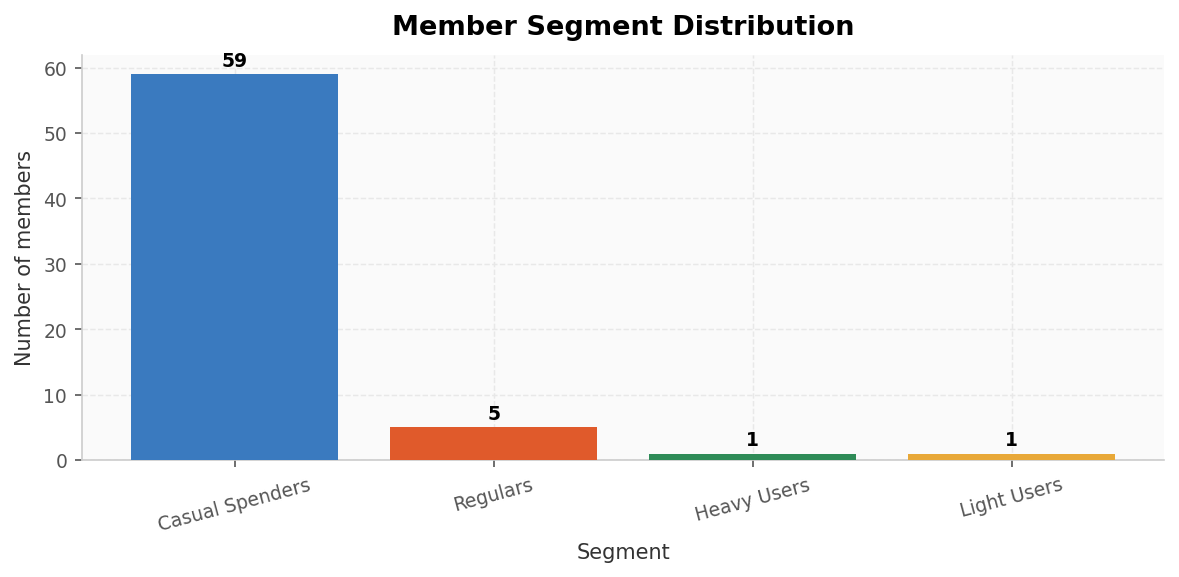
\includegraphics[width=0.80\textwidth]{segment_distribution.png}
  \caption{Number of members per segment.\label{fig:seg_dist}}
\end{figure}

\subsection{Continuous Loyalty Score}

Alongside the four discrete segments, 	exttt{segmenter.py} also exposes
	exttt{score\_member\_loyalty(dim\_member)}, a continuous per-member score
between 0 and 100 that blends three normalised signals: total spend, total
session time, and order activity. The score is written to
	exttt{output/forecasts/member\_loyalty.csv} together with a
	extit{loyalty\_tier} label (Bronze / Silver / Gold / Diamond) computed from
the score quartiles. Unlike the K-Means segmentation, which groups members by
behavioural profile, the loyalty score gives a single ordered ranking that the
chatbot uses when the owner asks ``who are my best customers?''.

\section{Anomaly Detection}

\subsection{Objective}

The anomaly detection module identifies days where one of three business metrics
deviated significantly from the normal pattern for that day of the week. The
output is a prioritised list of unusual dates for the owner to investigate, with
the most statistically extreme at the top.

\subsection{Why Day-of-Week Grouping}

A naive global Z-score (comparing each day to the overall dataset mean) would flag
every Saturday as anomalous, because Saturdays are consistently busier than
weekdays. That is not an anomaly; it is a regular pattern. The relevant question
is: was \textit{this particular Saturday} unusual compared to other Saturdays?

To answer that, the algorithm groups observations by day of the week and computes
the mean and standard deviation within each group independently. A day's score is
then how many standard deviations it falls from its weekday-specific mean:

\[
  Z = \frac{x - \mu_{\text{weekday}}}{\sigma_{\text{weekday}}}
\]

where $\mu_{\text{weekday}}$ is the mean of all values for the same day of the
week and $\sigma_{\text{weekday}}$ is their standard deviation. A minimum group
size of four is enforced; weekdays with fewer than four observations are skipped
to avoid unreliable Z-scores from very small samples.

\subsection{Three Monitored Series}

The function monitors three independent series simultaneously:

\begin{itemize}
  \item \textbf{Revenue}: total daily income from the cash transactions table.
  \item \textbf{Session volume}: number of transactions per day, used as a proxy
        for overall center activity.
  \item \textbf{Member activity}: number of member-type transactions per day.
\end{itemize}

\subsection{Severity Classification}

Days where $|Z| \geq 2.0$ are flagged. Two severity levels are defined:

\begin{itemize}
  \item \textbf{Mild}: $2.0 \leq |Z| < 3.0$. Noticeably unusual; worth reviewing
        in context.
  \item \textbf{Severe}: $|Z| \geq 3.0$. Highly unusual; likely reflects a real
        event such as a holiday, a promotional day, or a system issue.
\end{itemize}

Direction (\textit{high} or \textit{low}) is recorded separately so the owner
can distinguish between an unexpectedly strong day and an unexpectedly weak one.

No train/test split is applied. Unlike forecasting, which must be evaluated
prospectively, anomaly detection is a retrospective analysis of the complete
historical dataset: the goal is to surface what already happened, not to predict
what happens next.

\subsection{Output}

The function \texttt{detect\_anomalies()} in \texttt{gamefydb/anomaly\_detector.py}
writes \texttt{anomalies.csv} to \texttt{output/forecasts/}. Each row contains
the date, series name, day of the week, actual value, weekday mean and standard
deviation, Z-score, direction, and severity label. The output is sorted by
absolute Z-score descending, so the most extreme anomaly appears first.
Figure~\ref{fig:anomaly_timeline} shows what this looks like on the revenue series ---
mild anomalies in orange and severe ones in red on top of the daily revenue line.

\begin{figure}[H]
  \centering
  
\includegraphics[width=0.95\textwidth]{anomaly_timeline.png}
  \caption{Revenue anomaly timeline: daily revenue with mild (orange) and severe
           (red) anomaly markers.\label{fig:anomaly_timeline}}
\end{figure}

In Power~BI, this file powers a timeline visual overlaying anomaly markers on the
daily revenue chart.

\section{Output Summary}

All eight analytical outputs are written to \texttt{output/forecasts/} by
\texttt{run.py} at the end of every pipeline run.

\begin{table}[H]
  \centering
  \caption{Forecast output files and their Power~BI use.\label{tab:forecast_files}}
  \begin{tabular}{p{5cm} p{7.5cm}}
    \toprule
    \textbf{File} & \textbf{Use in Power~BI} \\
    \midrule
    \texttt{forecast\_revenue.csv}
      & Line chart showing projected revenue for the next 4 weeks and 3 months,
        with confidence band. \\[4pt]
    \texttt{forecast\_members.csv}
      & Bar or line chart showing projected member activity, useful for
        loyalty programme planning. \\[4pt]
    \texttt{peak\_hours\_by\_hour.csv}
      & Bar chart with hour (0--23) on X axis; shows hourly traffic pattern. \\[4pt]
    \texttt{peak\_hours\_by\_day.csv}
      & Bar chart with day name on X axis; shows weekly traffic pattern. \\[4pt]
    \texttt{session\_volume.csv}
      & Line chart showing projected total activity volume by week and month. \\[4pt]
    \texttt{stock\_replenishment.csv}
      & Table visual showing each item with its weekly consumption, suggested
        order quantity, and reorder frequency. \\[4pt]
    \texttt{member\_segments.csv}
      & Table or scatter chart showing each member with their segment label
        and feature values (lifetime TND, session duration, order spending). \\[4pt]
    \texttt{anomalies.csv}
      & Timeline visual overlaying anomaly markers on daily revenue; filterable
        by severity (mild or severe) and direction (high or low). \\
    \bottomrule
  \end{tabular}
\end{table}

\begin{figure}[H]
  \centering
  \fbox{\begin{minipage}{0.95\textwidth}\centering\vspace{3cm}
    \textit{[Screenshot: forecast visuals in Power~BI --- add \texttt{forecast\_powerbi.png}]}
  \vspace{3cm}\end{minipage}}
  \caption{Forecast visuals integrated into the Power~BI dashboard.\label{fig:forecast_pbi}}
\end{figure}

\section{Sprint 4 Review}

Before closing the sprint, each output was validated:

\begin{itemize}
  \item Revenue forecast: the 4-week projections were compared against the last
        four weeks of actual data to confirm magnitude and direction were plausible.
        The model correctly identified that weekends drive higher revenue.
  \item Member forecast: all \texttt{yhat\_lower} values were confirmed as
        non-negative integers throughout the forecast horizon.
  \item Peak hours: the missing hours 8 and 9 were confirmed as expected
        (no data, not an error). The \texttt{pct\_of\_total} column was confirmed
        to sum to exactly 100\% within each group.
  \item Stock replenishment: the suggested frequencies were reviewed with the
        Product Owner and confirmed to match his existing informal purchasing
        pattern for the high-velocity items.
  \item Member segmentation: the silhouette score was printed at runtime and
        confirmed as ACCEPTABLE or above. The four segment labels were reviewed
        with the Product Owner, who confirmed that the Heavy Users and Regulars
        segments matched his intuitive understanding of his most loyal members.
  \item Anomaly detection: the top five flagged dates by Z-score were reviewed.
        Each corresponded to an identifiable real event (a public holiday, a
        promotional weekend, or an unusually quiet day). No false positives were
        found among the severe-flagged dates.
\end{itemize}

\section{Conclusion}

Sprint~4 added a machine learning layer to a system that was previously only
descriptive. The five forecasting functions give the owner data-backed answers to
planning questions that previously required guesswork. The K-means segmentation
organises the member base into four interpretable groups that can drive targeted
loyalty actions. The anomaly detection module surfaces the days that deviated most
from expected patterns, giving the owner a prioritised list of dates to investigate.
These three analytics outputs are not the end of the project: Sprint~5 puts a
conversational assistant on top of them so the owner can read the forecasts,
segments, and anomaly flags as plain-language answers instead of CSV files.

% ============================================================
%  CHAPTER 7 — SPRINT 5
% ============================================================
\chapter{Sprint 5: Conversational Assistant}

\section{Introduction}

By the end of Sprint~4, the gaming centre had a star schema, a four-page
Power~BI report, and a full layer of forecasting, segmentation, and
anomaly detection. The numbers were all there. What was still missing was
a way for the owner to actually \emph{ask} a question without having to
remember which dashboard page hides which answer.

Sprint~5 closes that gap with a conversational assistant. The idea is
simple: the owner types (or speaks) a question in plain language --- in
English, French, or Arabic --- and the system replies with a written
answer and, when relevant, a chart. The assistant sits on top of the same
CSV outputs Power~BI consumes, so there is one source of truth.

\section{Sprint 5 Backlog}

Table~\ref{tab:sprint5_backlog} lists the tasks committed to this sprint.

\begin{longtable}{>{\bfseries}p{1.3cm} p{4.4cm} p{7cm}}
  \caption{Sprint 5 Backlog.\label{tab:sprint5_backlog}} \\
  \toprule
  \textbf{ID} & \textbf{User Story} & \textbf{Tasks} \\
  \midrule
  \endfirsthead
  \toprule
  \textbf{ID} & \textbf{User Story} & \textbf{Tasks} \\
  \midrule
  \endhead
  \bottomrule
  \endfoot

  US-18 & As an owner, I want to ask questions in plain language and get
          answers with charts.
        & Build a Streamlit front-end (\texttt{app.py}) wired to a Gemini-backed
          agent (\texttt{chatbot/agent.py}); load the star-schema and forecast
          CSVs as a shared \texttt{DataContext} (\texttt{chatbot/data\_loader.py}). \\[4pt]

  US-19 & As an owner, I want to use the assistant in English, French, or
          Arabic.
        & Translate the UI string bundle in \texttt{app.py} (\texttt{STRINGS}
          dict, three locales); pass a language instruction to the system
          prompt so the model also answers in the chosen language. \\[4pt]

  US-20 & As an owner, I want to talk to the assistant instead of typing.
        & Add a custom Streamlit component (\texttt{chatbot/voice\_component.py})
          backed by an HTML/JS frontend (\texttt{chatbot/voice\_html/}) that
          uses the browser's Web Speech API; pass the selected language as
          the recognition locale (\texttt{en-US}, \texttt{fr-FR}, or \texttt{ar-TN}). \\[4pt]

  US-21 & As an owner, I want a chart drawn on demand when one would help.
        & Implement \texttt{chatbot/chart\_generator.py} on top of Plotly
          Express; have the agent emit a structured \texttt{chart\_spec}
          JSON block when a chart is useful and render it in the right
          panel of the layout. \\
\end{longtable}

\section{Architecture Overview}

Sprint~5 adds a fifth layer on top of the four-layer pipeline introduced
in Sprint~0. Figure~\ref{fig:chatbot_arch} sketches the flow at runtime.

\begin{figure}[H]
  \centering
  % *TODO* Render a sequence/arch diagram for the chatbot. Suggested boxes:
  % User -> Streamlit (app.py) -> [DataContext (CSVs)] + [voice_component]
  %       -> agent.ask() -> Gemini API -> agent._parse_response() -> chart_generator
  %       -> Plotly figure + answer + suggestions -> back to Streamlit.
  
\includegraphics[width=0.92\textwidth]{images/chatbot_arch.png}
  \caption{Runtime architecture of the conversational assistant.}
  \label{fig:chatbot_arch}
\end{figure}

The pieces are intentionally small. The Streamlit app owns the layout, the
session state, and the language toggle. The agent module owns the prompt
construction and the model call. The chart generator turns a
\texttt{chart\_spec} into a Plotly figure. The voice component is a thin
wrapper around a browser API. The data loader reads the CSV outputs of
the previous sprints into a single in-memory \texttt{DataContext} that the
agent passes to the model as schema + summary text.

\section{Implementation}

\subsection{Loading the Data Context}

\texttt{chatbot/data\_loader.py} reads eleven CSV files into a shared
\texttt{DataContext} dataclass:

\begin{itemize}[noitemsep]
  \item From \texttt{output/powerbi\_star/}: \texttt{fact\_transaction},
        \texttt{fact\_session}, \texttt{dim\_member}.
  \item From \texttt{output/forecasts/}: \texttt{forecast\_revenue},
        \texttt{session\_volume}, \texttt{member\_segments},
        \texttt{member\_loyalty}, \texttt{anomalies},
        \texttt{peak\_hours\_by\_hour}, \texttt{peak\_hours\_by\_day},
        \texttt{stock\_replenishment}.
\end{itemize}

For each table the loader emits a short schema line (column names plus
dtypes) and aggregates a one-shot summary string: total revenue, member
count, loyalty-tier distribution, the next four weekly and three monthly
revenue forecasts, recent-anomaly count, average session duration, and
session-type breakdown. The two strings (\texttt{schemas} and
\texttt{summary}) are spliced into the system prompt at every turn so the
model always has both the structure of the data and the headline numbers
in front of it.

A useful side effect: the loader also exposes a
\texttt{recent\_anomaly\_count()} helper, so the Streamlit app can change
its startup greeting when something interesting has happened in the
previous seven days.

\subsection{The Conversational Agent}

\texttt{chatbot/agent.py} is the bridge between the Streamlit app and
the Gemini API. It does three things:

\begin{enumerate}
  \item \textbf{Build the system prompt.} The prompt mixes a fixed
        instruction block, the language directive, the schema string, and
        the summary string. The instructions tell the model to answer
        concisely, to include a single \texttt{chart\_spec} JSON block
        only when a chart would actually help, to suggest two or three
        follow-up questions, to refuse questions that cannot be answered
        from the available data, and to never invent numbers.
  \item \textbf{Call the model.} The full conversation history is
        re-sent on every turn (Gemini \texttt{gemini-3-flash-preview}),
        with the system prompt attached as
        \texttt{system\_instruction}. The model returns one piece of
        free text that contains the answer and, optionally, two JSON
        code blocks.
  \item \textbf{Parse the response.} A small regex pass extracts the
        \texttt{chart\_spec} block and the \texttt{suggestions} block,
        then strips them out of the visible answer so the chat shows
        clean prose only.
\end{enumerate}

The system prompt also contains a short ``source selection rules''
section that nudges the model towards the right table for each kind of
question (revenue trend $\to$ \texttt{fact\_transaction}; future
revenue $\to$ \texttt{forecast\_revenue} with a granularity filter;
hourly pattern $\to$ \texttt{peak\_hours\_by\_hour}; and so on). This
turned out to matter more than tuning the temperature. Without the rules,
the model would happily plot \texttt{fact\_session} on a non-existent
date axis or use the \texttt{anomalies} table for generic revenue
questions.

\subsection{Chart Generation}

\texttt{chatbot/chart\_generator.py} converts a \texttt{chart\_spec} dict
into a Plotly Express figure. The spec is small on purpose --- just
\texttt{type}, \texttt{x}, \texttt{y}, \texttt{source} (the table key),
\texttt{filter} (a pandas \texttt{query} expression that the agent can
fill in), and \texttt{title}. Four chart types are supported:
\textit{bar}, \textit{line}, \textit{scatter}, and \textit{pie}. If the
\texttt{y} column is non-numeric, the generator groups by \texttt{x} and
counts instead of trying to aggregate a string column. A dark theme is
applied to match the rest of the Streamlit layout.

Charts are not rendered when the model decides one is not useful (for
example, ``how many members do I have in total?'' returns a one-line
answer with no figure). This keeps the right-hand panel meaningful
instead of being filled with redundant visuals.

\subsection{Voice Input}

\texttt{chatbot/voice\_component.py} declares a custom Streamlit
component pointing at a small HTML/JS frontend in
\texttt{chatbot/voice\_html/}. The frontend uses the browser's
\texttt{SpeechRecognition} API to capture audio, transcribe it locally
in the browser, and post the transcript back to Streamlit. The selected
language toggle is forwarded to the component as a recognition locale
(\texttt{en-US}, \texttt{fr-FR}, or \texttt{ar-TN}), so French users
get French transcription and Arabic users get Tunisian-Arabic
transcription out of the box.

Keeping the recognition in the browser avoids having to wire a separate
speech-to-text service, and means voice mode works offline once the page
is loaded.

\subsection{Multilingual UI}

The \texttt{STRINGS} dictionary in \texttt{app.py} carries every visible
label in three languages. Switching language flips the dict, sends a new
language directive into the system prompt, and updates the voice
component's recognition locale --- all in one place, all without
reloading the data. The Arabic strings are stored as-is, and Streamlit
renders them right-to-left where appropriate.

The greeting is also context-aware. If the anomaly detector flagged
something in the previous seven days, the assistant opens with
``I noticed \texttt{N} anomaly(ies) in the past 7 days. Want me to show
you?'' instead of the generic ``Hi! Ask me anything.'' This tiny detail
was the change that made the assistant feel most useful in practice:
the owner does not have to think to discover that something is off.

\subsection{Quick Actions}

Four shortcut buttons sit under the chat history --- \textit{Full
summary}, \textit{Give me advice}, \textit{Any anomalies?}, and
\textit{Forecast}. Each one just enqueues a pre-written prompt into
\texttt{st.session\_state.pending\_query} and triggers a rerun, so the
model receives the question as if the user had typed it. They cover the
three or four questions the owner asks most often, and skip the typing
cost.

\section{Sprint 5 Review}

\subsection{Deliverables}

\begin{itemize}[noitemsep]
  \item \texttt{app.py} --- 252-line Streamlit application: language
        toggle, anomaly-aware greeting, chat panel with suggestion
        chips, chart panel, quick-action buttons, voice button.
  \item \texttt{chatbot/agent.py} --- prompt builder, Gemini call, and
        structured-response parser.
  \item \texttt{chatbot/chart\_generator.py} --- Plotly-Express
        renderer for the four supported chart types.
  \item \texttt{chatbot/data\_loader.py} --- shared
        \texttt{DataContext}, schema/summary builder,
        \texttt{recent\_anomaly\_count()} helper.
  \item \texttt{chatbot/voice\_component.py} +
        \texttt{chatbot/voice\_html/} --- browser-side speech
        recognition wired into Streamlit.
\end{itemize}

\subsection{Validation}

The assistant was validated against three kinds of questions:

\begin{itemize}
  \item \textbf{Descriptive} --- ``Which cashier had the best March?'',
        ``What is the average session duration?'', ``Show me revenue by
        payment method.'' Answers and charts matched the corresponding
        Power~BI page on every test case.
  \item \textbf{Forecast} --- ``How much revenue should I expect next
        month?'', ``Will members grow in May?'' Returned the values
        from \texttt{forecast\_revenue.csv} and
        \texttt{session\_volume.csv} with the right granularity filter.
  \item \textbf{Anomaly} --- ``Anything unusual last week?'' Returned
        the rows from \texttt{anomalies.csv} flagged within the
        seven-day window, matching the \texttt{recent\_anomaly\_count}
        helper.
\end{itemize}

The multilingual handling was checked end-to-end: a French question
produced a French answer with the chart title in French, and an Arabic
question produced an Arabic answer rendered right-to-left.

\section{Conclusion}

Sprint~5 turned a folder of CSV files into something the owner can
actually \emph{converse} with. There is no new data in the system ---
the agent reads exactly the same outputs the dashboards do --- but the
interaction model is fundamentally different. Instead of clicking
through four dashboard pages to answer a question, the owner asks the
question. Instead of remembering which CSV holds the anomaly list, the
greeting brings the answer to him. The chatbot is the practical face
of every previous sprint: without the cleaning, the schema, the
dashboards, and the ML layer it would have nothing to talk about, but
without the chatbot none of those would have been accessible without
opening Power~BI. The next chapter wraps up the project as a whole.

% ============================================================
%  GENERAL CONCLUSION
% ============================================================
\chapter*{General Conclusion}
\addcontentsline{toc}{chapter}{General Conclusion}

This project started from a simple observation: a gaming center that records
everything but analyses nothing. Four months later, the result is a system that
automatically transforms four raw Excel files into a clean data warehouse, four
interactive dashboards, five forward-looking forecasts, one member segmentation,
one anomaly detection report, and a conversational AI assistant that answers
business questions in English, French, or Arabic.

The technical work divided naturally into two parts. The ETL work in Sprints~1 and 2
was the less visible but more foundational half. Discovering that the source files
contained page-break artefacts, non-standard number formats, column shifts from
merged cells, and cashier naming inconsistencies (none of it documented) took up
most of Sprint~1. None of this was documented anywhere, so most of it had to be
figured out by loading the files, looking at what came out, and working backwards
from there. A dashboard built on top of uncleaned data would have shown wrong
numbers with no indication that anything was off, which seemed like a worse
outcome than having no dashboard at all.
Sprint~2 then assembled the six-table star schema from the clean DataFrames, a
process that also required one design revision: reducing from eight tables to six
when it became clear that the stock and member data were better represented as
dimensions than as fact tables.

Sprint~3 turned the star schema into four dashboard pages in Power~BI. The
design went through a few iterations before the owner was satisfied --- the
Live Ops page in particular was reorganised after the first review because
the stock table was not visible without scrolling. The final version was
validated by the Product Owner and can be refreshed by re-running the pipeline
whenever new source files are available.

Sprint~4 was added after Sprint~3 was validated because the Product Owner wanted
to know not just what had happened but what to expect next. The forecasting part
took the most time --- choosing between Prophet, SARIMA, and XGBoost, running the
evaluations, and then dealing with the fact that the test window fell right in the
middle of Ramadan, which the model had never seen before. The April 2026 validation
was added later specifically to show that outside of that period the model actually
performs reasonably well. The K-means segmentation and anomaly detection were more
straightforward by comparison, though getting the cluster labels to be stable and
interpretable required some iteration on the feature selection.

Sprint~5 was the last piece. By that point everything the system needed to
\emph{know} was already in the CSVs --- what was missing was a way for the owner to
\emph{ask}. A Streamlit assistant backed by the Gemini API, with multilingual
support (English, French, Arabic) and a voice-input mode, sits on top of the same
data Power~BI consumes. The greeting becomes anomaly-aware when something has been
flagged in the previous seven days, so the most pressing information surfaces on
its own. Building the chatbot was the smallest sprint in code volume but probably
the most visible one to the Product Owner --- it is the layer that turns the rest
of the system into something he uses every day rather than something he opens
when he has the time.

Forecast accuracy was validated against April 2026 actuals: Prophet predicted the
month's total revenue within 5.4\% (8{,}389 TND predicted vs 7{,}959 TND actual),
and weekly errors ranged from 6\% to 25\%, confirming that the model is useful for
real operational decisions. The higher daily MAPE (64\%) reflects a data-coverage
gap --- Ramadan 2025 predates the dataset, so the model had never seen that pattern
before --- rather than a fundamental modelling weakness.

There are several directions worth exploring in a future iteration. The most
practically valuable would be connecting the pipeline directly to the management
software's database rather than relying on periodic Excel exports, which would allow
automatic daily refreshes. The Prophet models would benefit from a second calendar
year of data: the current ten-month window is enough to detect weekly patterns
reliably, but twelve more months would let the models learn yearly seasonality and
handle recurring events such as Ramadan without the data-gap problem documented in
Section~\ref{sec:april_validation}.

Looking back, the part that took the most effort was also the least visible:
getting the raw Excel files into a consistent, usable format. By the time the
dashboards were built, most of the hard decisions had already been made at the
cleaning and schema design stage. The machine learning sprint was probably
the most uncertain in terms of whether it would produce anything useful ---
a 64\% daily MAPE is not a number you want to present, and understanding why
it happened (Ramadan, missing history) took some time to work through. The April
validation helped put that result in context. Overall the system does what it was
supposed to do, and the owner now has tools he can actually use without needing
a data analyst present.

% ============================================================
%  BIBLIOGRAPHY
% ============================================================
\chapter*{Bibliography}
\addcontentsline{toc}{chapter}{Bibliography}

\begin{thebibliography}{99}

\bibitem{prophet}
Taylor, S.J. and Letham, B. (2018).
\textit{Forecasting at scale}.
The American Statistician, 72(1), 37--45.
\url{https://doi.org/10.1080/00031305.2017.1380080}

\bibitem{kimball}
Kimball, R. and Ross, M. (2013).
\textit{The Data Warehouse Toolkit: The Definitive Guide to Dimensional Modeling}.
3rd edition. Wiley.

\bibitem{inmon}
Inmon, W.H. (2005).
\textit{Building the Data Warehouse}.
4th edition. Wiley.

\bibitem{scrum}
Schwaber, K. and Sutherland, J. (2020).
\textit{The Scrum Guide: The Definitive Guide to Scrum: The Rules of the Game}.
Scrum.org. \url{https://scrumguides.org}

\bibitem{pandas}
McKinney, W. (2010).
Data Structures for Statistical Computing in Python.
\textit{Proceedings of the 9th Python in Science Conference}, 56--61.

\bibitem{powerbi}
Microsoft Corporation (2024).
\textit{Power BI documentation}.
\url{https://learn.microsoft.com/en-us/power-bi/}

\bibitem{dax}
Ferrari, A. and Russo, M. (2019).
\textit{The Definitive Guide to DAX: Business intelligence for Microsoft Power BI,
SQL Server Analysis Services, and Excel}.
2nd edition. Microsoft Press.

\bibitem{gimsi}
Fernandez, A. (2002).
\textit{Le projet décisionnel: de la modélisation à la mise en œuvre}.
Eyrolles.

\bibitem{numpy}
Harris, C.R. et al. (2020).
Array programming with NumPy.
\textit{Nature}, 585, 357--362.
\url{https://doi.org/10.1038/s41586-020-2649-2}

\end{thebibliography}

\end{document}
